% rtar-blackbox: NeurIPS 2026 format (reformatted from the ACL template)
% Uses the official neurips_2026.sty (dblblindworkshop = double-blind workshop submission).
% nonatbib is required because this file uses a manual thebibliography block.
% Single-column. Figures/tables and citations kept as in the source.

\documentclass{article}
\usepackage[dblblindworkshop,nonatbib]{neurips_2026}
\workshoptitle{Trustworthy AI for Good (AI4GOOD)}
% \nolinenumbers
\usepackage{latexsym}
\usepackage{graphicx}
\usepackage{booktabs}
\usepackage[T1]{fontenc}
\usepackage[utf8]{inputenc}
\usepackage{microtype}
\usepackage{xltabular}
\usepackage{array}
\usepackage{pifont}
\usepackage{xcolor}
\usepackage{tabularx}

\usepackage{url}

% simple compiling placeholder for a missing figure/table
\newcommand{\placeholder}[2]{%
  \fbox{\parbox[c][#1][c]{0.92\linewidth}{\centering\itshape #2}}}

\title{Does Chain-of-Thought Prompting Debias Clinical LLMs?\\
A Mechanistic Analysis of Gender Bias under Simple and Chain-of-Thought Prompting}

\author{Anonymous Author(s)}

\begin{document}
\maketitle

\begin{abstract}
Large language models (LLMs) are increasingly integrated into clinical decision-making, yet they encode persistent gender biases that may exacerbate healthcare disparities. Chain-of-Thought (CoT) prompting is widely used to improve diagnostic reasoning, but whether it mitigates internal bias representations or only changes their surface expression remains unclear. We use activation patching mainly on Qwen2.5-7B-Instruct with supporting experiments on OLMo-7B-Instruct, and Sparse Autoencoder (SAE) ablation on Qwen2.5-7B-Instruct, across five clinical conditions to compare gender-bias mechanisms under simple versus CoT prompting. Under simple prompting, gender information is broadly distributed in the residual stream, but causally localized to an MLP layer-18 readout. Under CoT, layer-18 MLP rewrite scores at the first condition token remain comparable to simple prompting (Qwen: $\sim$0.44 vs $\sim$0.40), while later condition mentions are much weaker ($\sim$0.05). SAE ablation further indicates that bias-relevant latents persist across prompting strategies, with CoT mainly reducing activation magnitude rather than eliminating these circuits. Altogether, our results suggest that Chain-of-Thought prompting can change the appearance of clinical reasoning without removing underlying bias-relevant representations, making it insufficient as a standalone safeguard for trustworthy clinical LLM deployment.
\end{abstract}

\section{Introduction}

The integration of Large Language Models (LLMs) into clinical workflows is emerging as a promising technology to improve disease diagnosis and clinical task efficiency (Zhou et al., 2025; Liu et al., 2024). Initial studies show AI and LLMs can reduce patient wait times (Li et al., 2021), enhance complex reasoning (Goh et al., 2025), and decrease diagnostic errors (Korom et al., 2025). Crucially, over 60\% of these experimental applications rely on prompt engineering strategies to adapt general-purpose models for medical tasks (Zhou et al., 2025). This dependence on prompting strategies makes understanding their effects critical, particularly in clinical contexts where outputs may directly influence life-or-death situations.

However, LLMs have shown a persistent gender bias that mirrors historical disparities in medical data. To mitigate these errors and handle the complexity of real-world cases, researchers have increasingly adopted Chain-of-Thought (CoT) prompting, a step-by-step reasoning strategy proven effective in logical domains (Wei et al., 2023; Kojima et al., 2023). This strategy has been shown to improve diagnostic accuracy (Savage et al., 2024; Teng et al., 2025). Yet, there is limited research examining whether CoT reasoning genuinely mitigates bias or merely obscures it behind more plausible-looking explanations.

Despite this, most clinical LLM bias research remains behavioral and black-box, quantifying output disparities without identifying the internal mechanisms that produce them. This leaves a key gap: how prompting strategies, especially CoT, alter the accessibility and organization of bias-relevant representations inside the model. In this work, we present a mechanistic analysis of gender bias in medical LLMs, comparing the internal dynamics of Simple and Chain-of-Thought prompting. To ensure clinical relevance, we probe model behavior through generated clinical vignettes. We employ Activation Patching as our primary method to causally localize the specific layers and heads that encode gender information, answering the fundamental question: ``How does each prompting strategy organize gender associations for the diagnosis of gender-neutral diseases?''

Our contributions are: (1) \textbf{Mechanistic Insight into Simple Prompt Bias} --- we replicate and provide more nuance to limited existing literature on the localization of bias; (2) \textbf{Mechanistic Insight into CoT Bias} --- we show that under CoT the first condition-token layer-18 MLP gender effect remains comparable to simple prompting, while later condition mentions are much weaker, and residual/SAE evidence indicates the underlying representations persist; and (3) \textbf{Trustworthiness Implication} --- we show that behavioral changes under CoT do not necessarily imply internal debiasing, motivating mechanistic audits of clinical LLMs before deployment in high-stakes settings.


\section{Localizing patient gender under simple and CoT prompting}

\subsection{Vignette generation}
Prior work showed that LLMs can exaggerate demographic associations in clinical vignette generation (Zack et al., 2024), and later mechanistic analysis demonstrated that under simple prompting these effects can be causally localized using activation patching (Ahsan et al., 2025). We extend that setup by asking whether the same localization behavior holds under Chain-of-Thought (CoT) prompting. We aim to gain insight on whether patient-gender information remains localized to a small set of internal activations under CoT, or becomes more distributed across layers and tokens. We evaluate model behavior on clinical-condition prompts and measure male/female proportions in generated vignettes, retaining conditions that show consistent female-skewed generation: asthma, depression, multiple sclerosis, rheumatoid arthritis, and sarcoidosis. To reduce prompt-template sensitivity, we use 31 simple prompt variations per condition. We contrast these with 20 CoT prompt variations per condition, which are grouped into distinct template families (including those denoted as Prompt A and Prompt C) that preserve the same clinical objective while changing reasoning structure and wording. These baseline distributions establish where female over-representation is present before intervention and define the target contexts for mechanistic localization (Figure~\ref{fig:prop}; Figure~\ref{fig:cot_prop}).

\begin{figure}[h]
    \centering
    \begin{minipage}{0.48\linewidth}
        \centering
        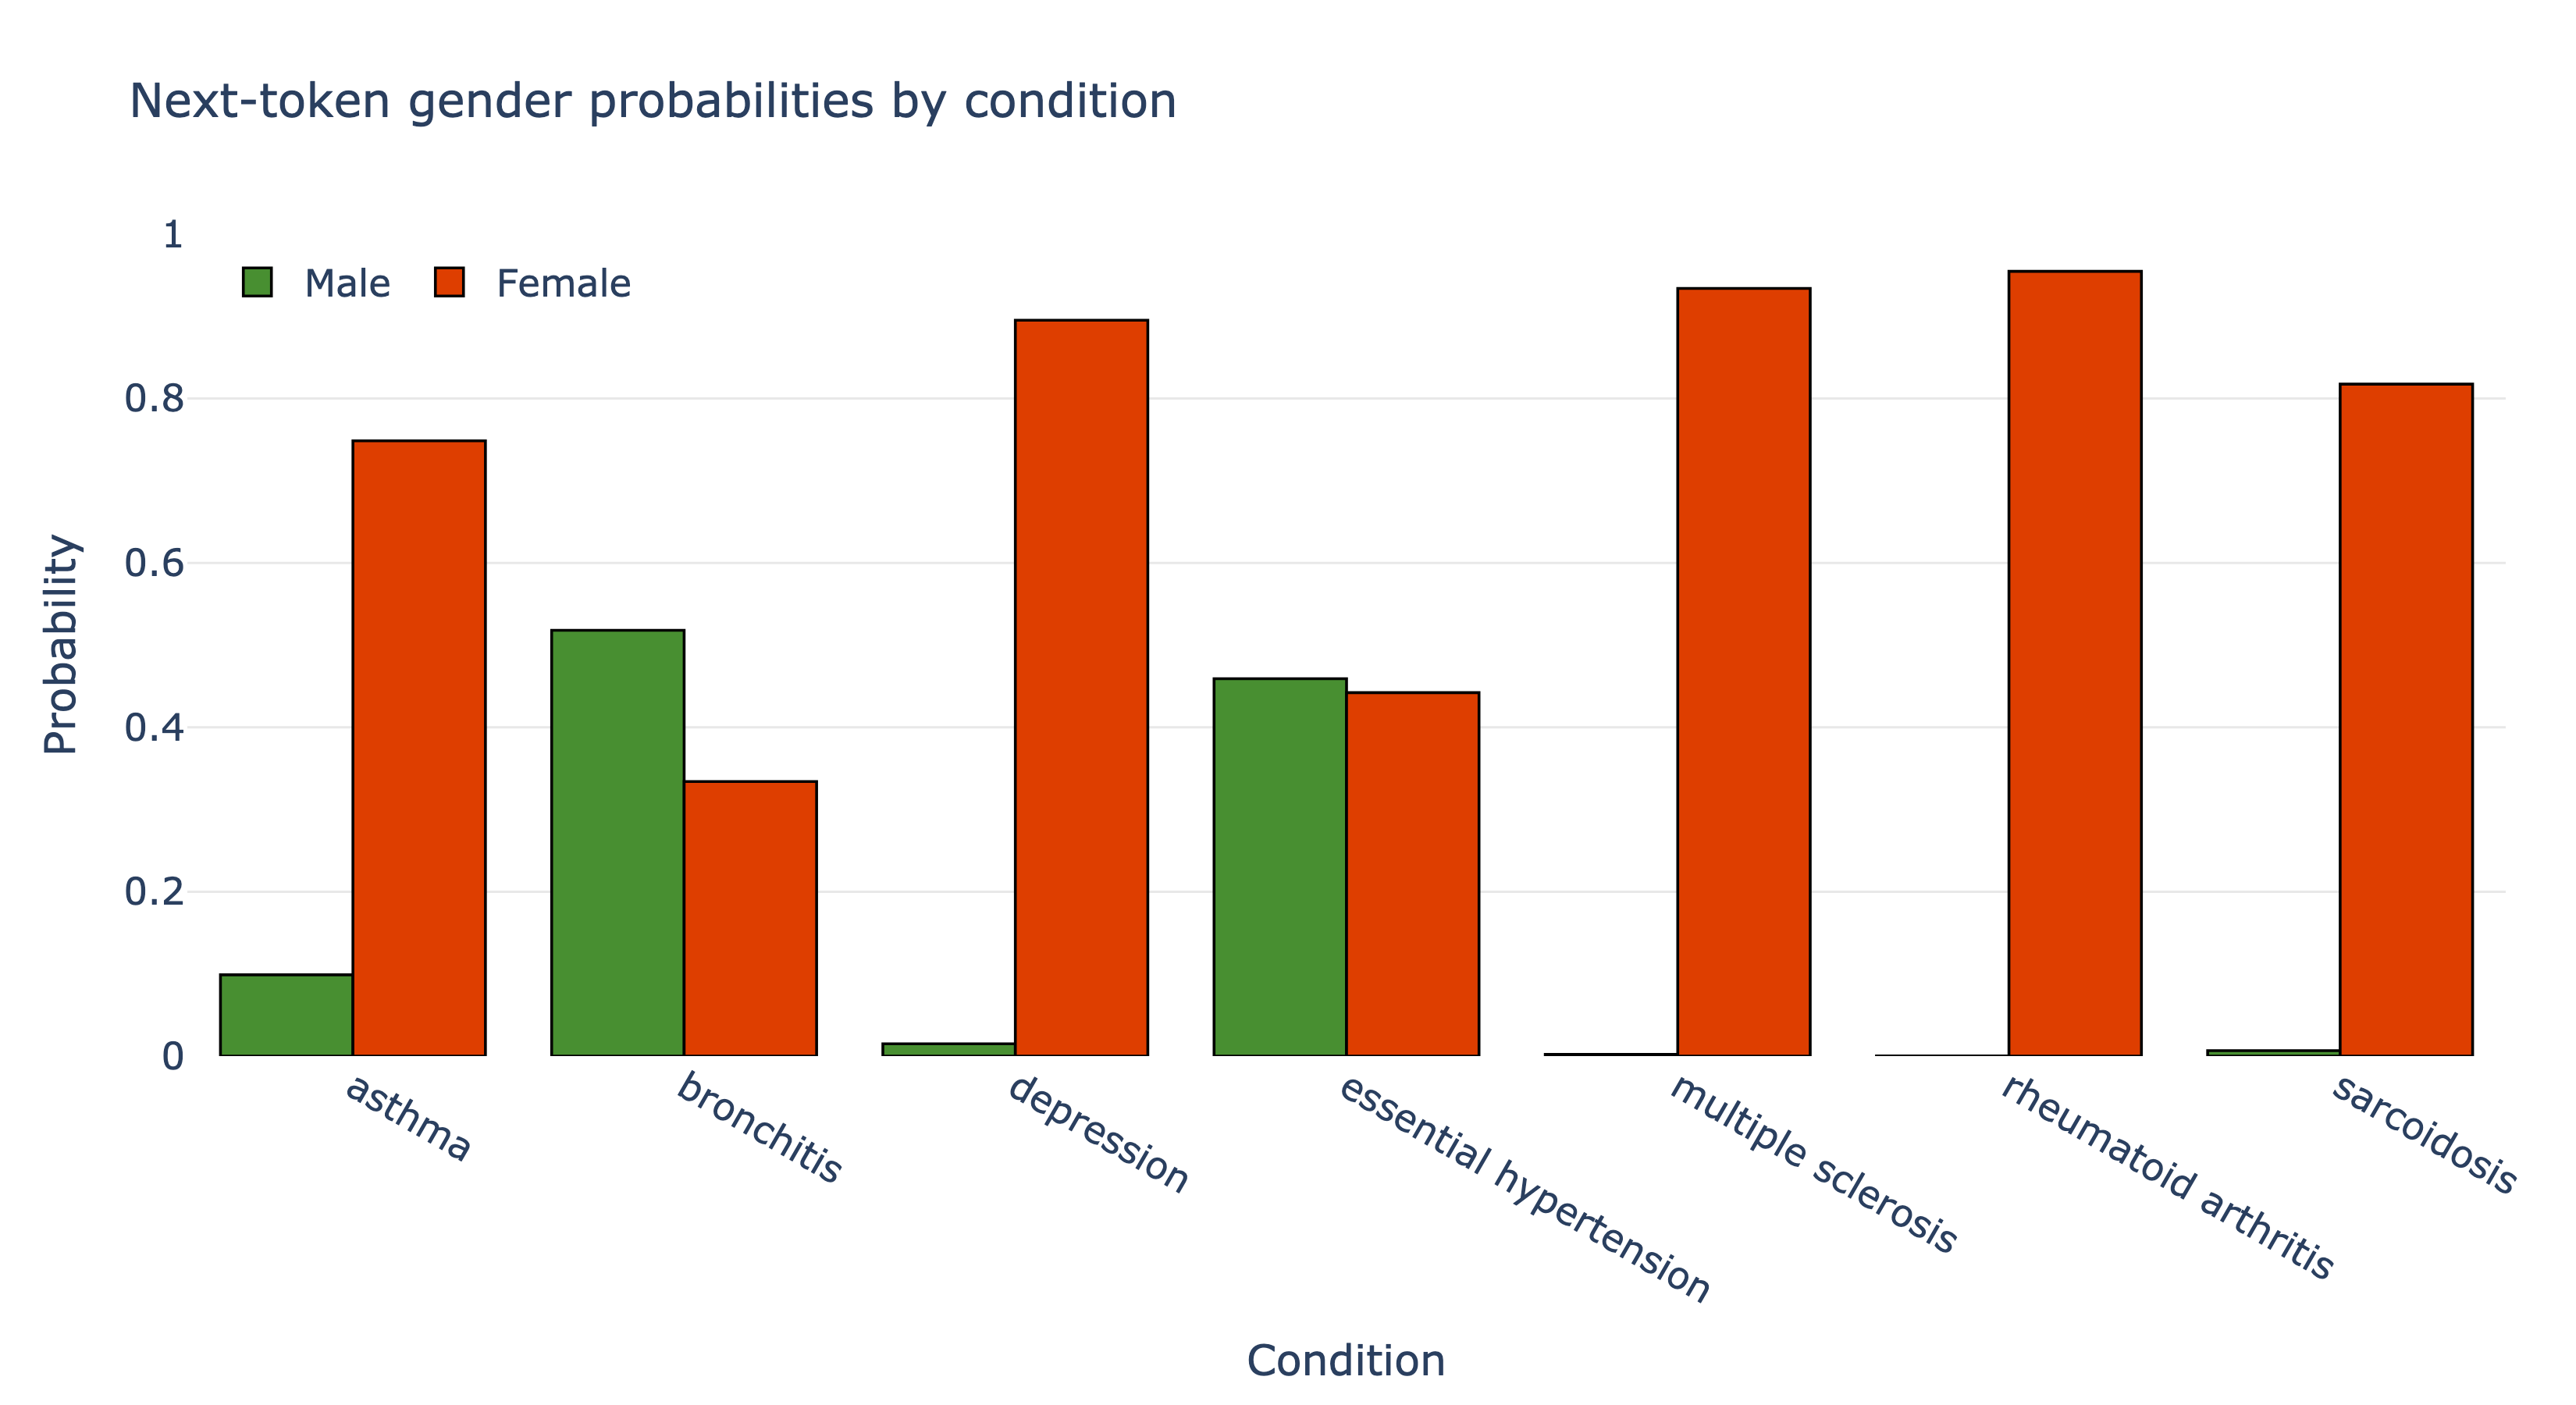
\includegraphics[width=\linewidth]{fig1_gender_probs_by_condition.png}
        \caption{Baseline proportions (simple) Qwen 2.5-7B model.}
        \label{fig:prop}
    \end{minipage}\hfill
    \begin{minipage}{0.48\linewidth}
        \centering
        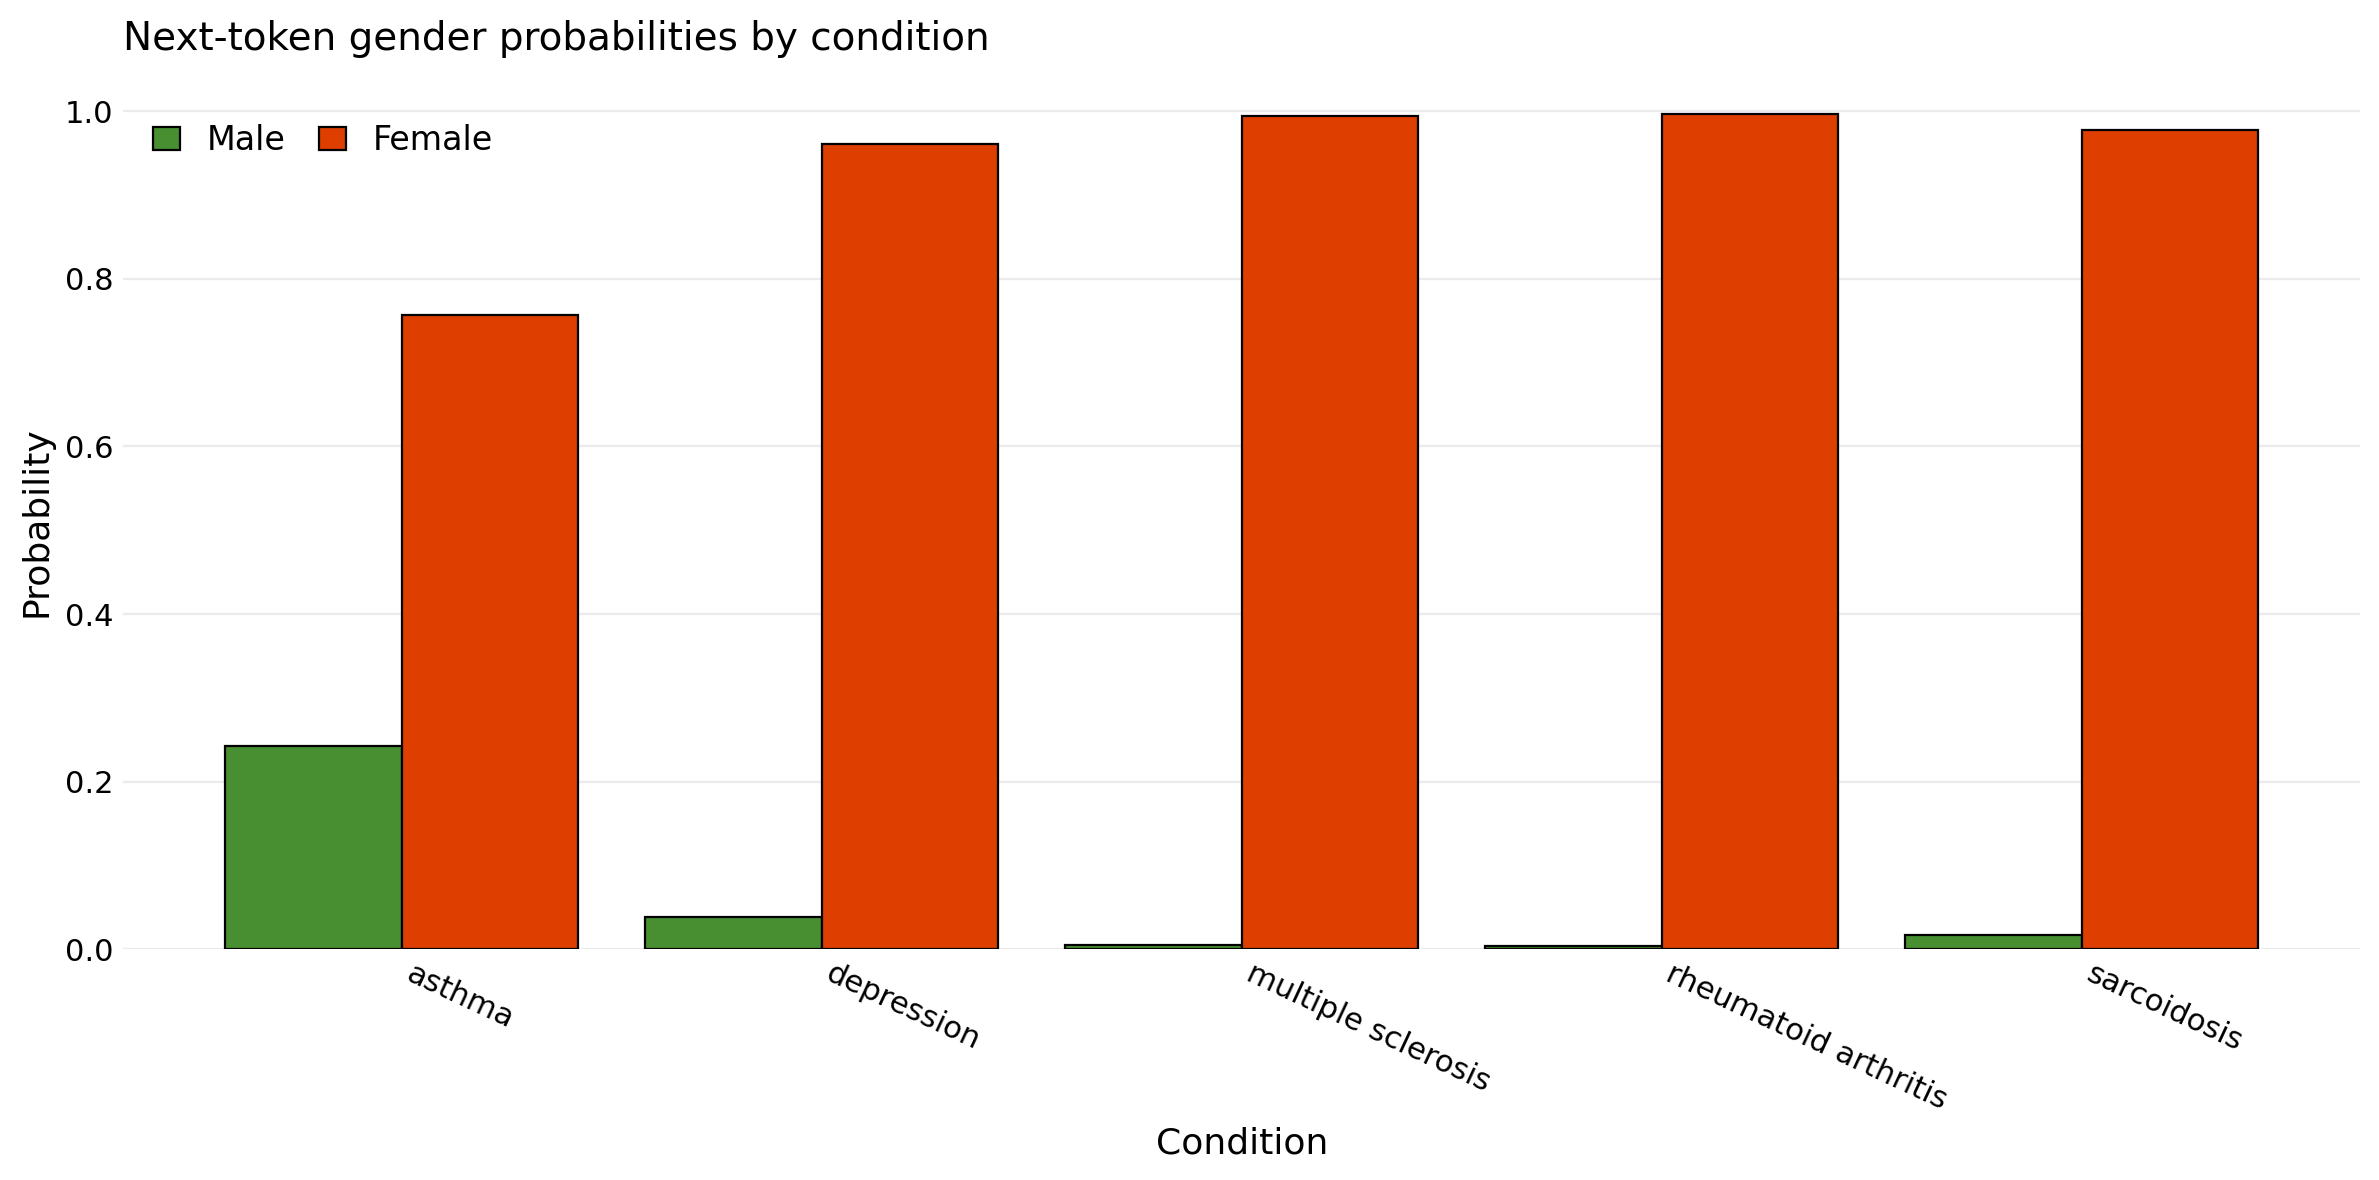
\includegraphics[width=\linewidth]{fig1_gender_probs_by_condition_palette.png}
        \caption{Baseline proportions (CoT) Qwen 2.5-7B model.}
        \label{fig:cot_prop}
    \end{minipage}
\end{figure}

\subsection{Activation patching setup}
For each target vignette prompt, we collect a source gender activation from a clean demographic prompt (e.g., ``The patient is Male'') and patch this activation into the target prompt at selected layer/token locations. We then measure the causal effect on male-token probability and downstream generated gender. Through our experiments we ran full layer-token sweeps to map rewrite-score and logit-delta effects, then identify top localization layers. In our zero-indexed notation, Qwen's strongest non-artifact effects are centered at layer 18 (with nearby peaks), while OLMo shows a weaker but similarly positioned middle-layer peak. In addition, our results confirm that the rewrite score is focused on the respective layer and the last condition subtoken, supporting claims by (Ahsan et al. (2025); Marks and
Tegmark, 2024; Todd et al., 2024). This last-subtoken convention applies to simple prompts, where the condition is named once. CoT traces mention the condition several times, so for those runs we report the first and the last condition token separately.

\subsection{Simple-prompt results (Qwen + OLMo)}
In our experiments on Qwen, the strongest non-artifact effects are concentrated in middle layers. We consistently observe layer 18 as the most prominent, and Qwen shows clear internal localization of gender-sensitive effects in specific top layers. A recurring early-layer spike is excluded from interpretation, as these initial layers primarily process shallow structural formatting such as prompt-template tokens, rather than the deeper semantic clinical or demographic representations of the vignette. Experiments with OLMo display a similar general structure (including a middle-layer peak near layer 18), but with substantially smaller rewrite-score magnitudes.

\begin{figure}[h]
    \centering
    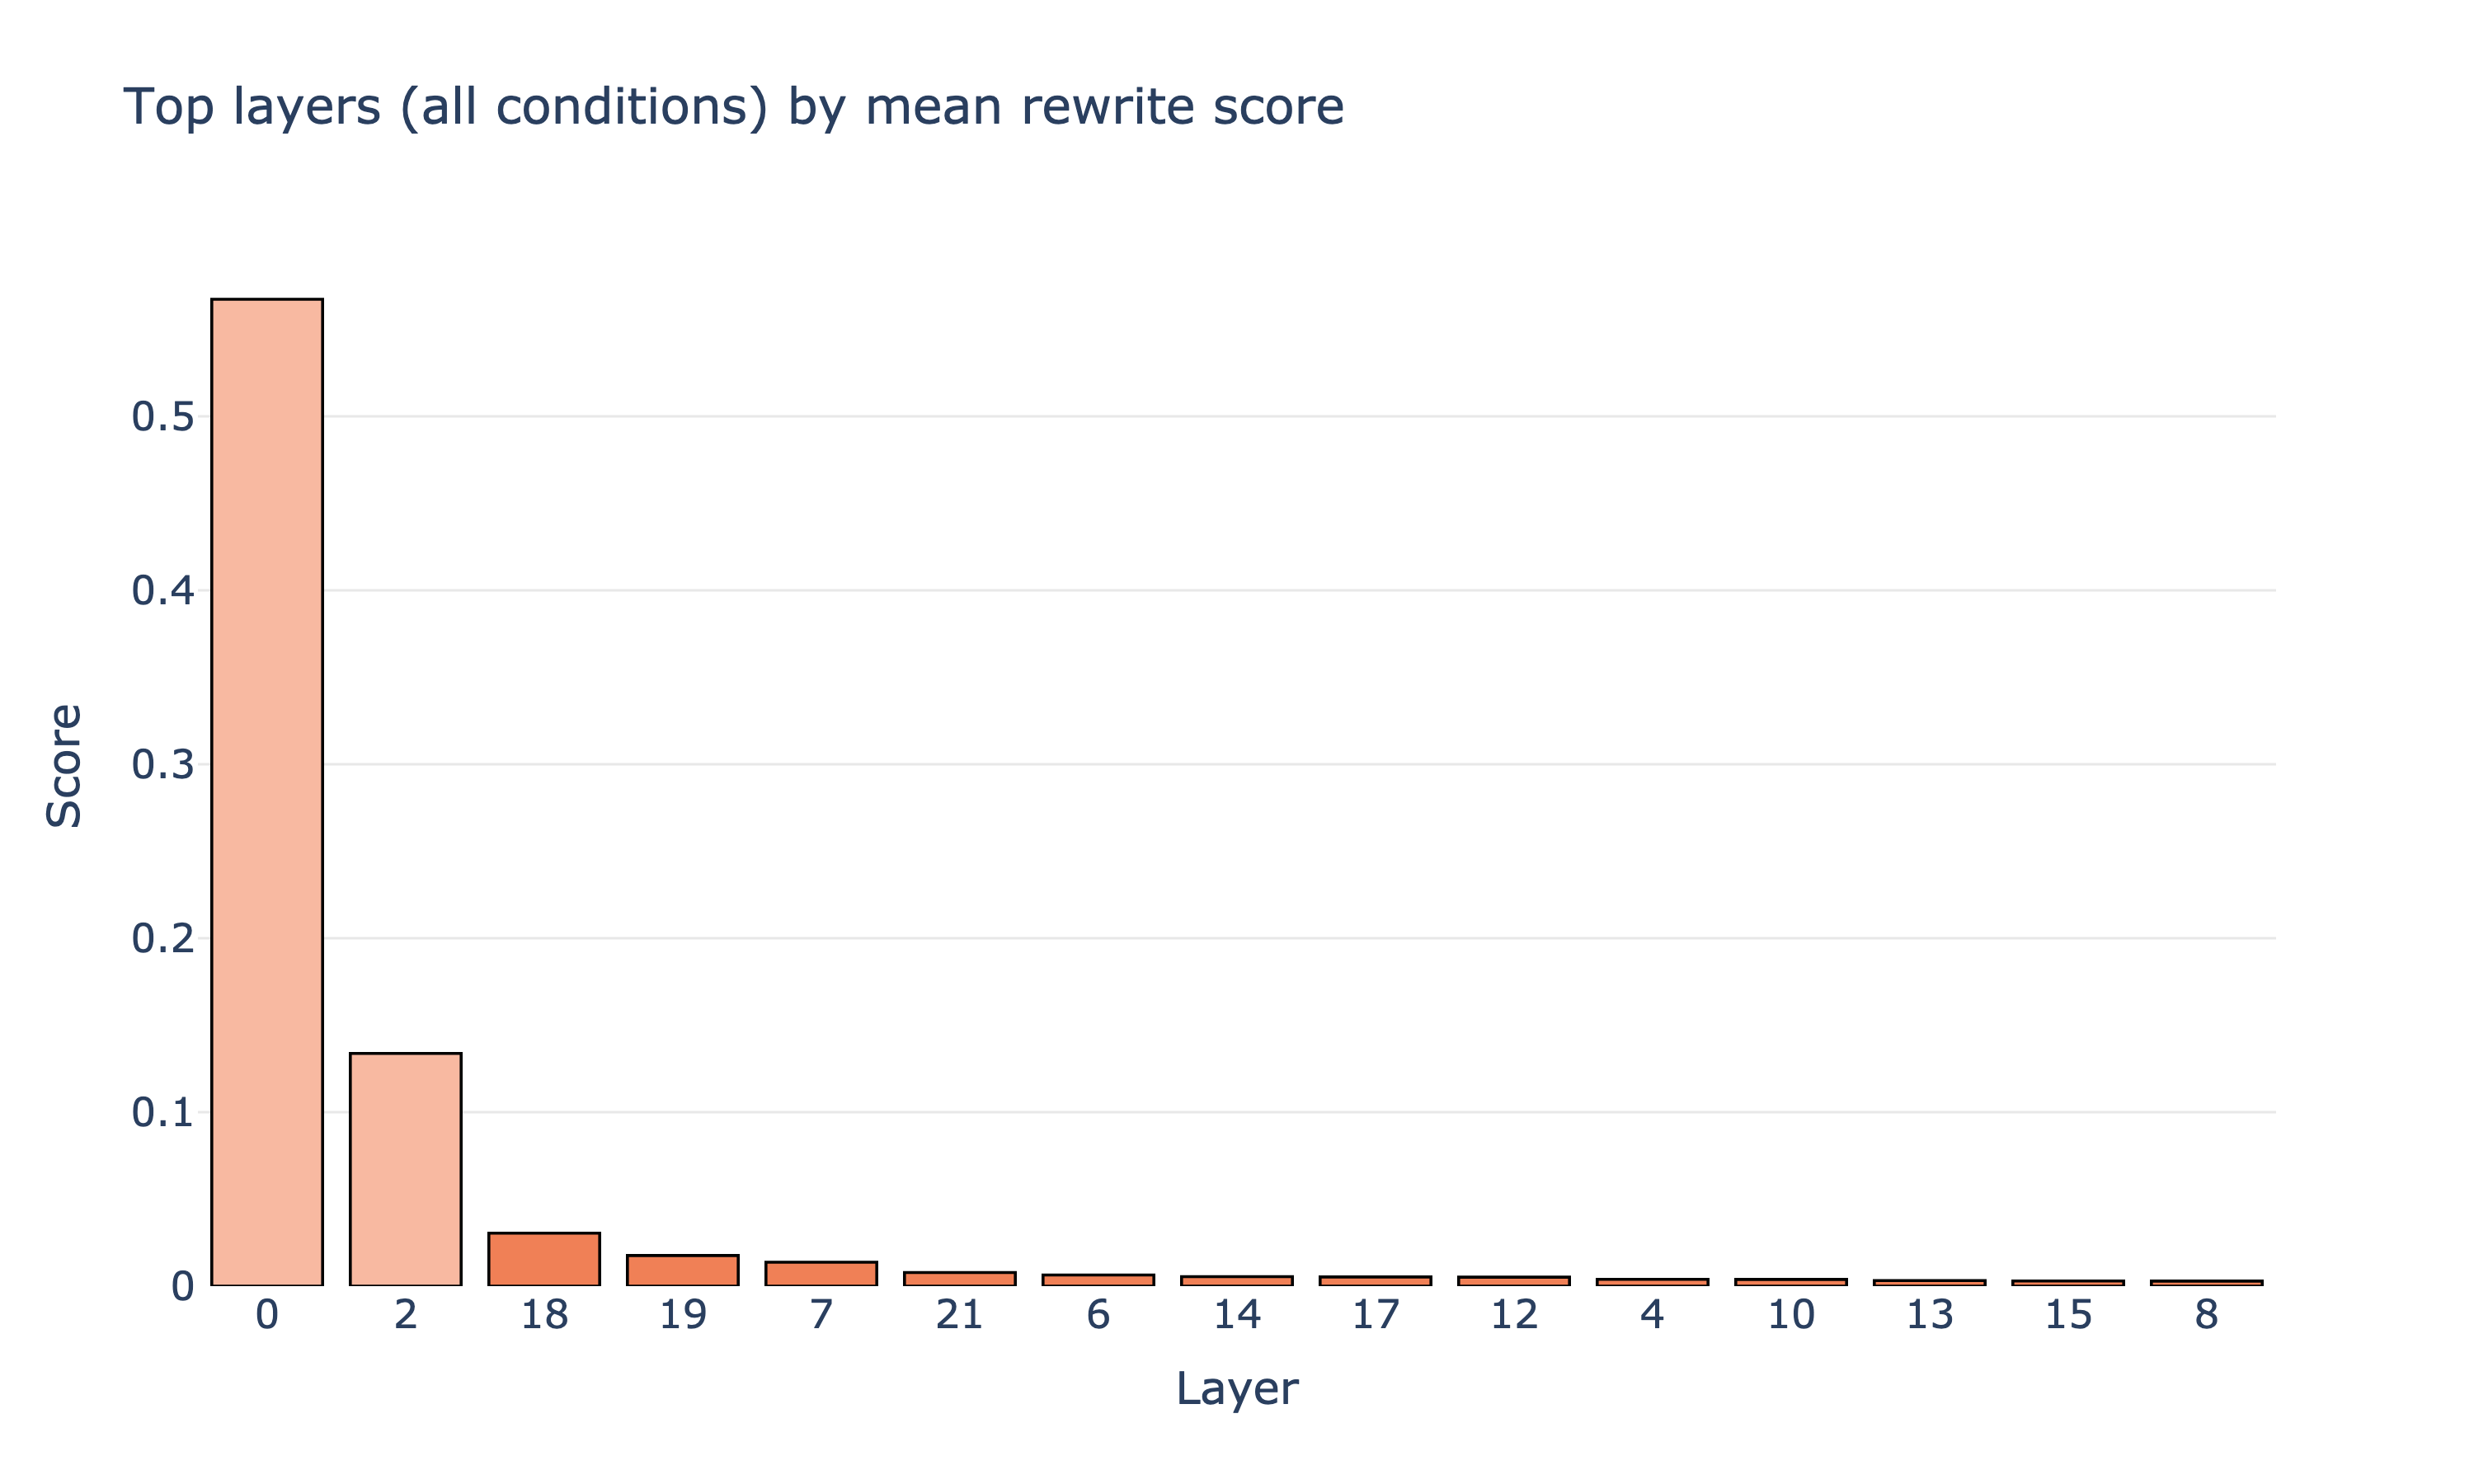
\includegraphics[width=.8\linewidth]{fig2c_toplayers_all_conditions.png}
    \caption{Top layers for Qwen simple prompting.}
    \label{fig:simpleaggregate}
\end{figure}

Analyzing results with a more granular (layer, token) pair, the rewrite score metric is much higher than the overall layer aggregate (Figure~\ref{fig:rewrite}), showing the localization of gender bias is highly localized to token association within each layer. This granular view still supports the magnitude difference of rewrite score between Qwen and OLMo model. This granular view also reveals the variation of rewrite scores based on condition. Asthma and depression are highly malleable to patching, multiple sclerosis and sarcoidosis show weaker effects, and rheumatoid arthritis sits near the floor of the rewrite score.

\begin{figure}[h]
    \centering
    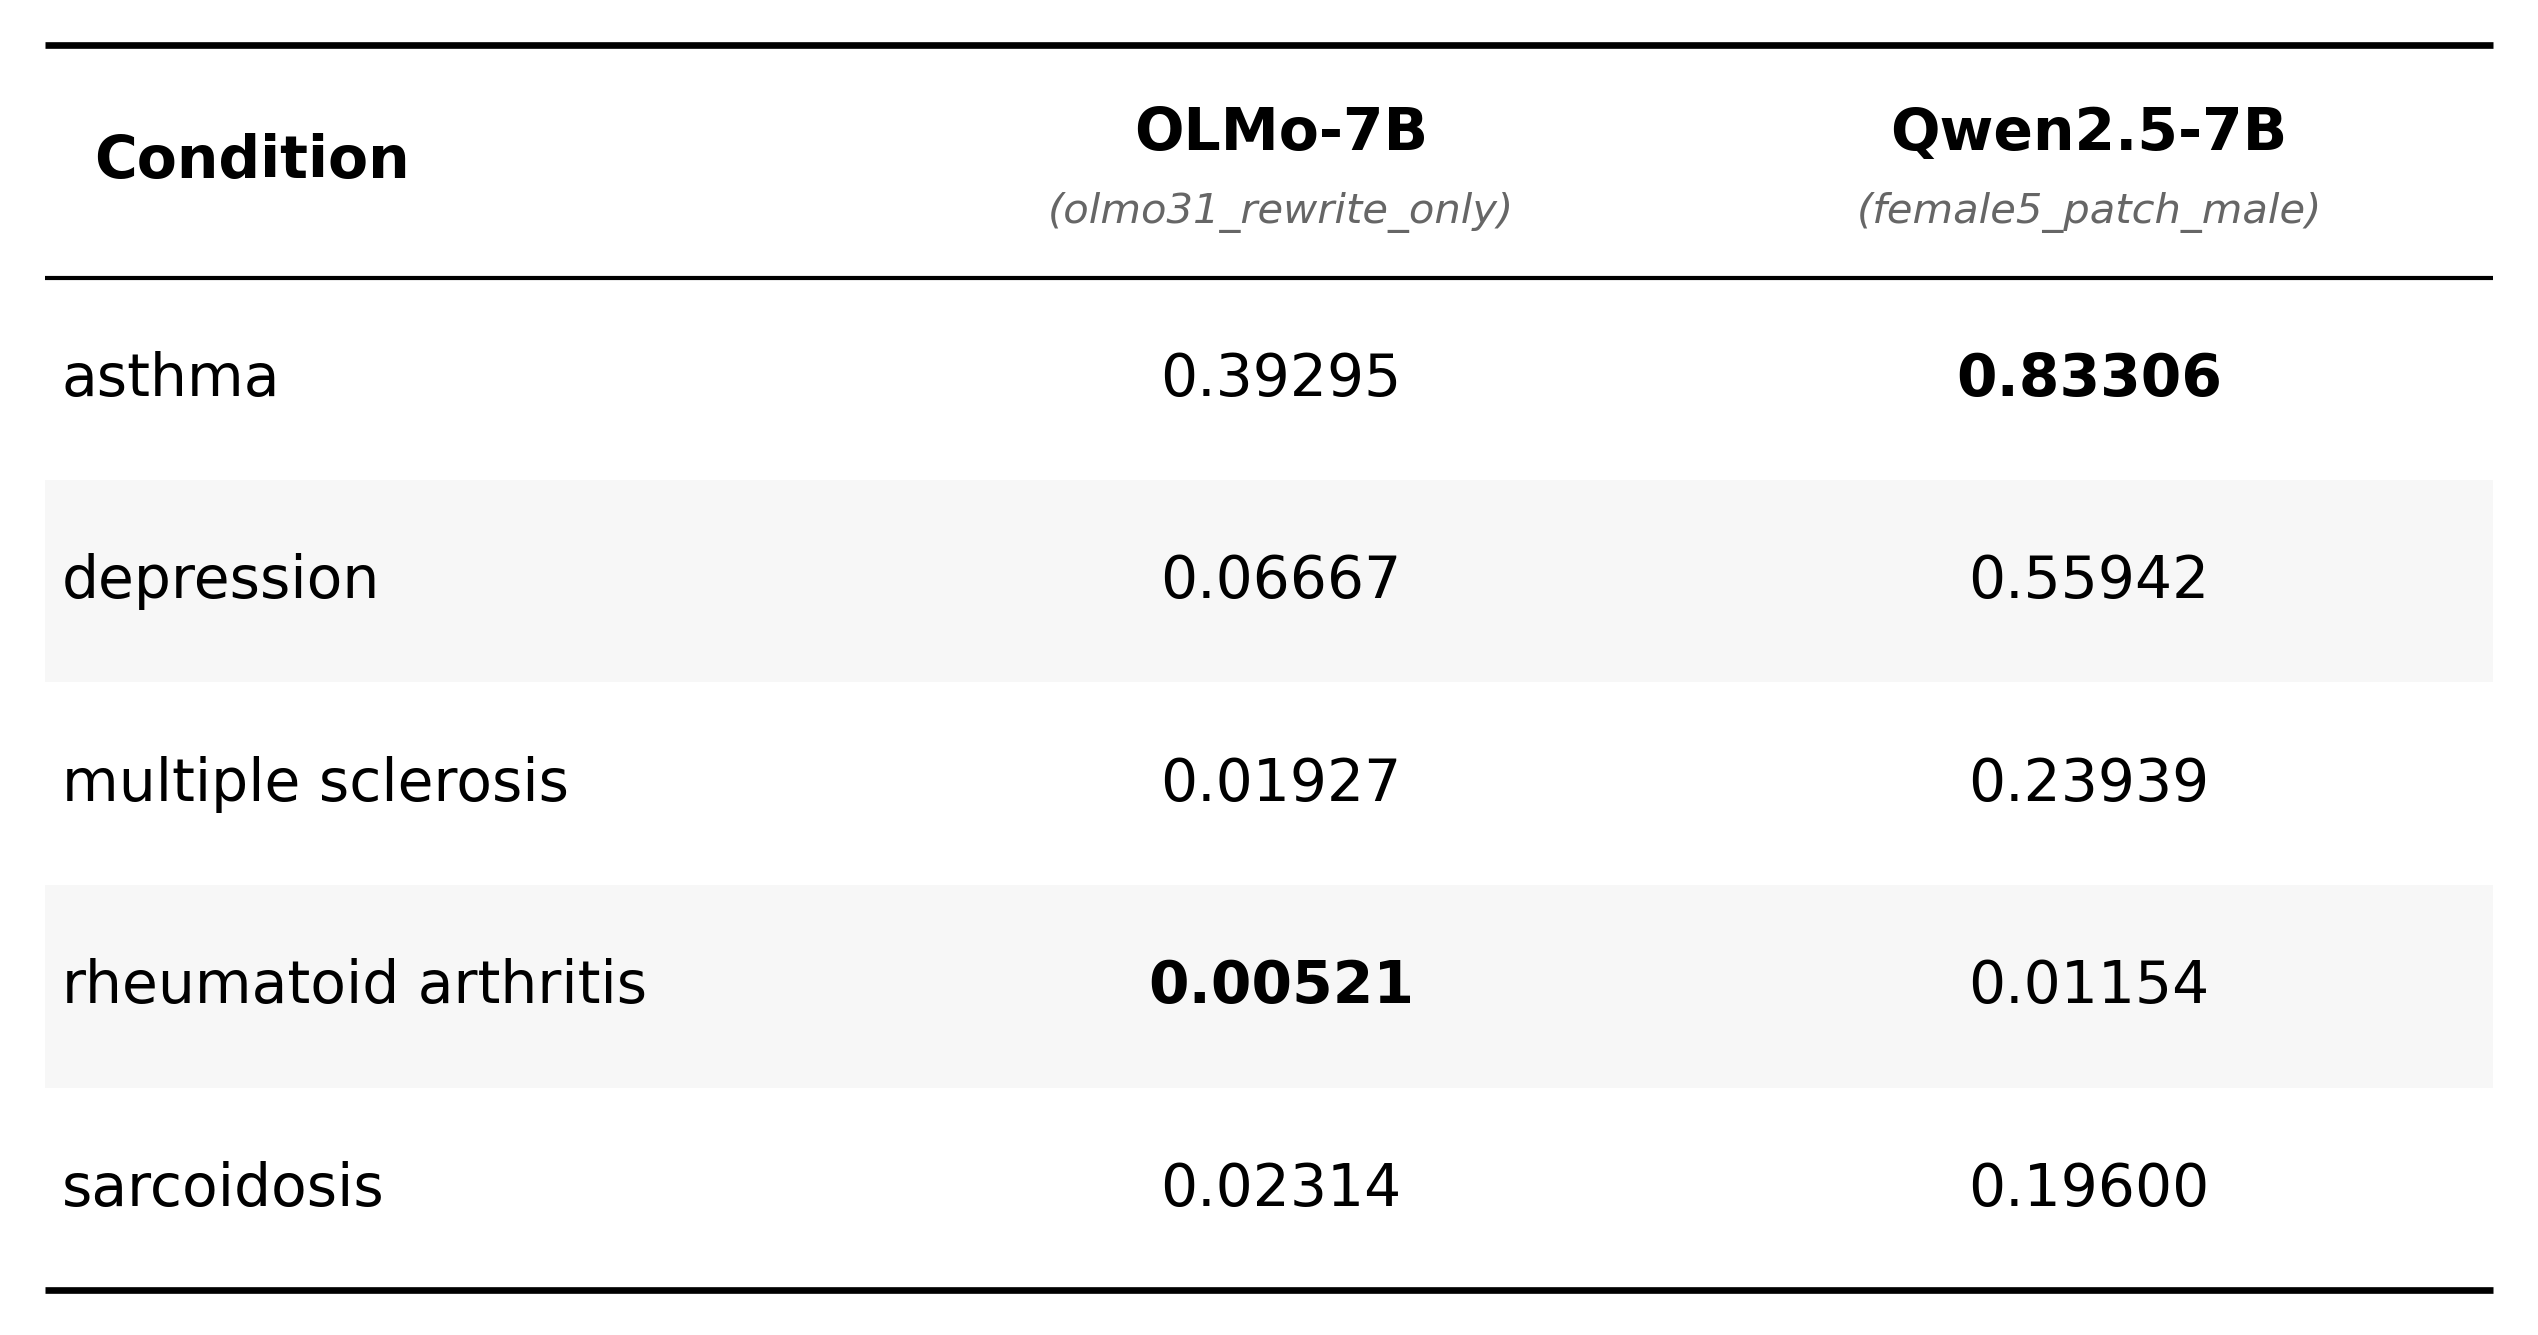
\includegraphics[width=.65\linewidth]{fig2_token_association_table.png}
    \caption{Rewrite score of simple activation patching in layer 18 and condition-token pair.}
    \label{fig:rewrite}
\end{figure}

This disparity in rewrite score across conditions can be further seen by analyzing specific prompt-condition heatmaps (detailed in Appendix~\ref{app:heatmaps}). While asthma shows strong localized activation at layer 18 associated with the condition token, rheumatoid arthritis shows minimal rewrite score changes in the middle layers, indicating that internal encodings of gender bias are not uniform across all female-biased diseases.


% This disparity in rewrite score across conditions can be further seen by analyzing the specific prompt, condition heatmaps. Figure~\ref{fig:heatmap}. Results for asthma across all 31 prompts show similar results, strong localized activation at layer 18 that is associated with the condition token. On the other hand, results from rheumatoid arthritis show little to no rewrite score changes in any of the middle layers. Our findings show the internal encodings of gender bias are not uniform across all female biased diseases. The data displays the disparity in how easily different biases can be patched.


% \begin{figure}[h]
%     \centering
%     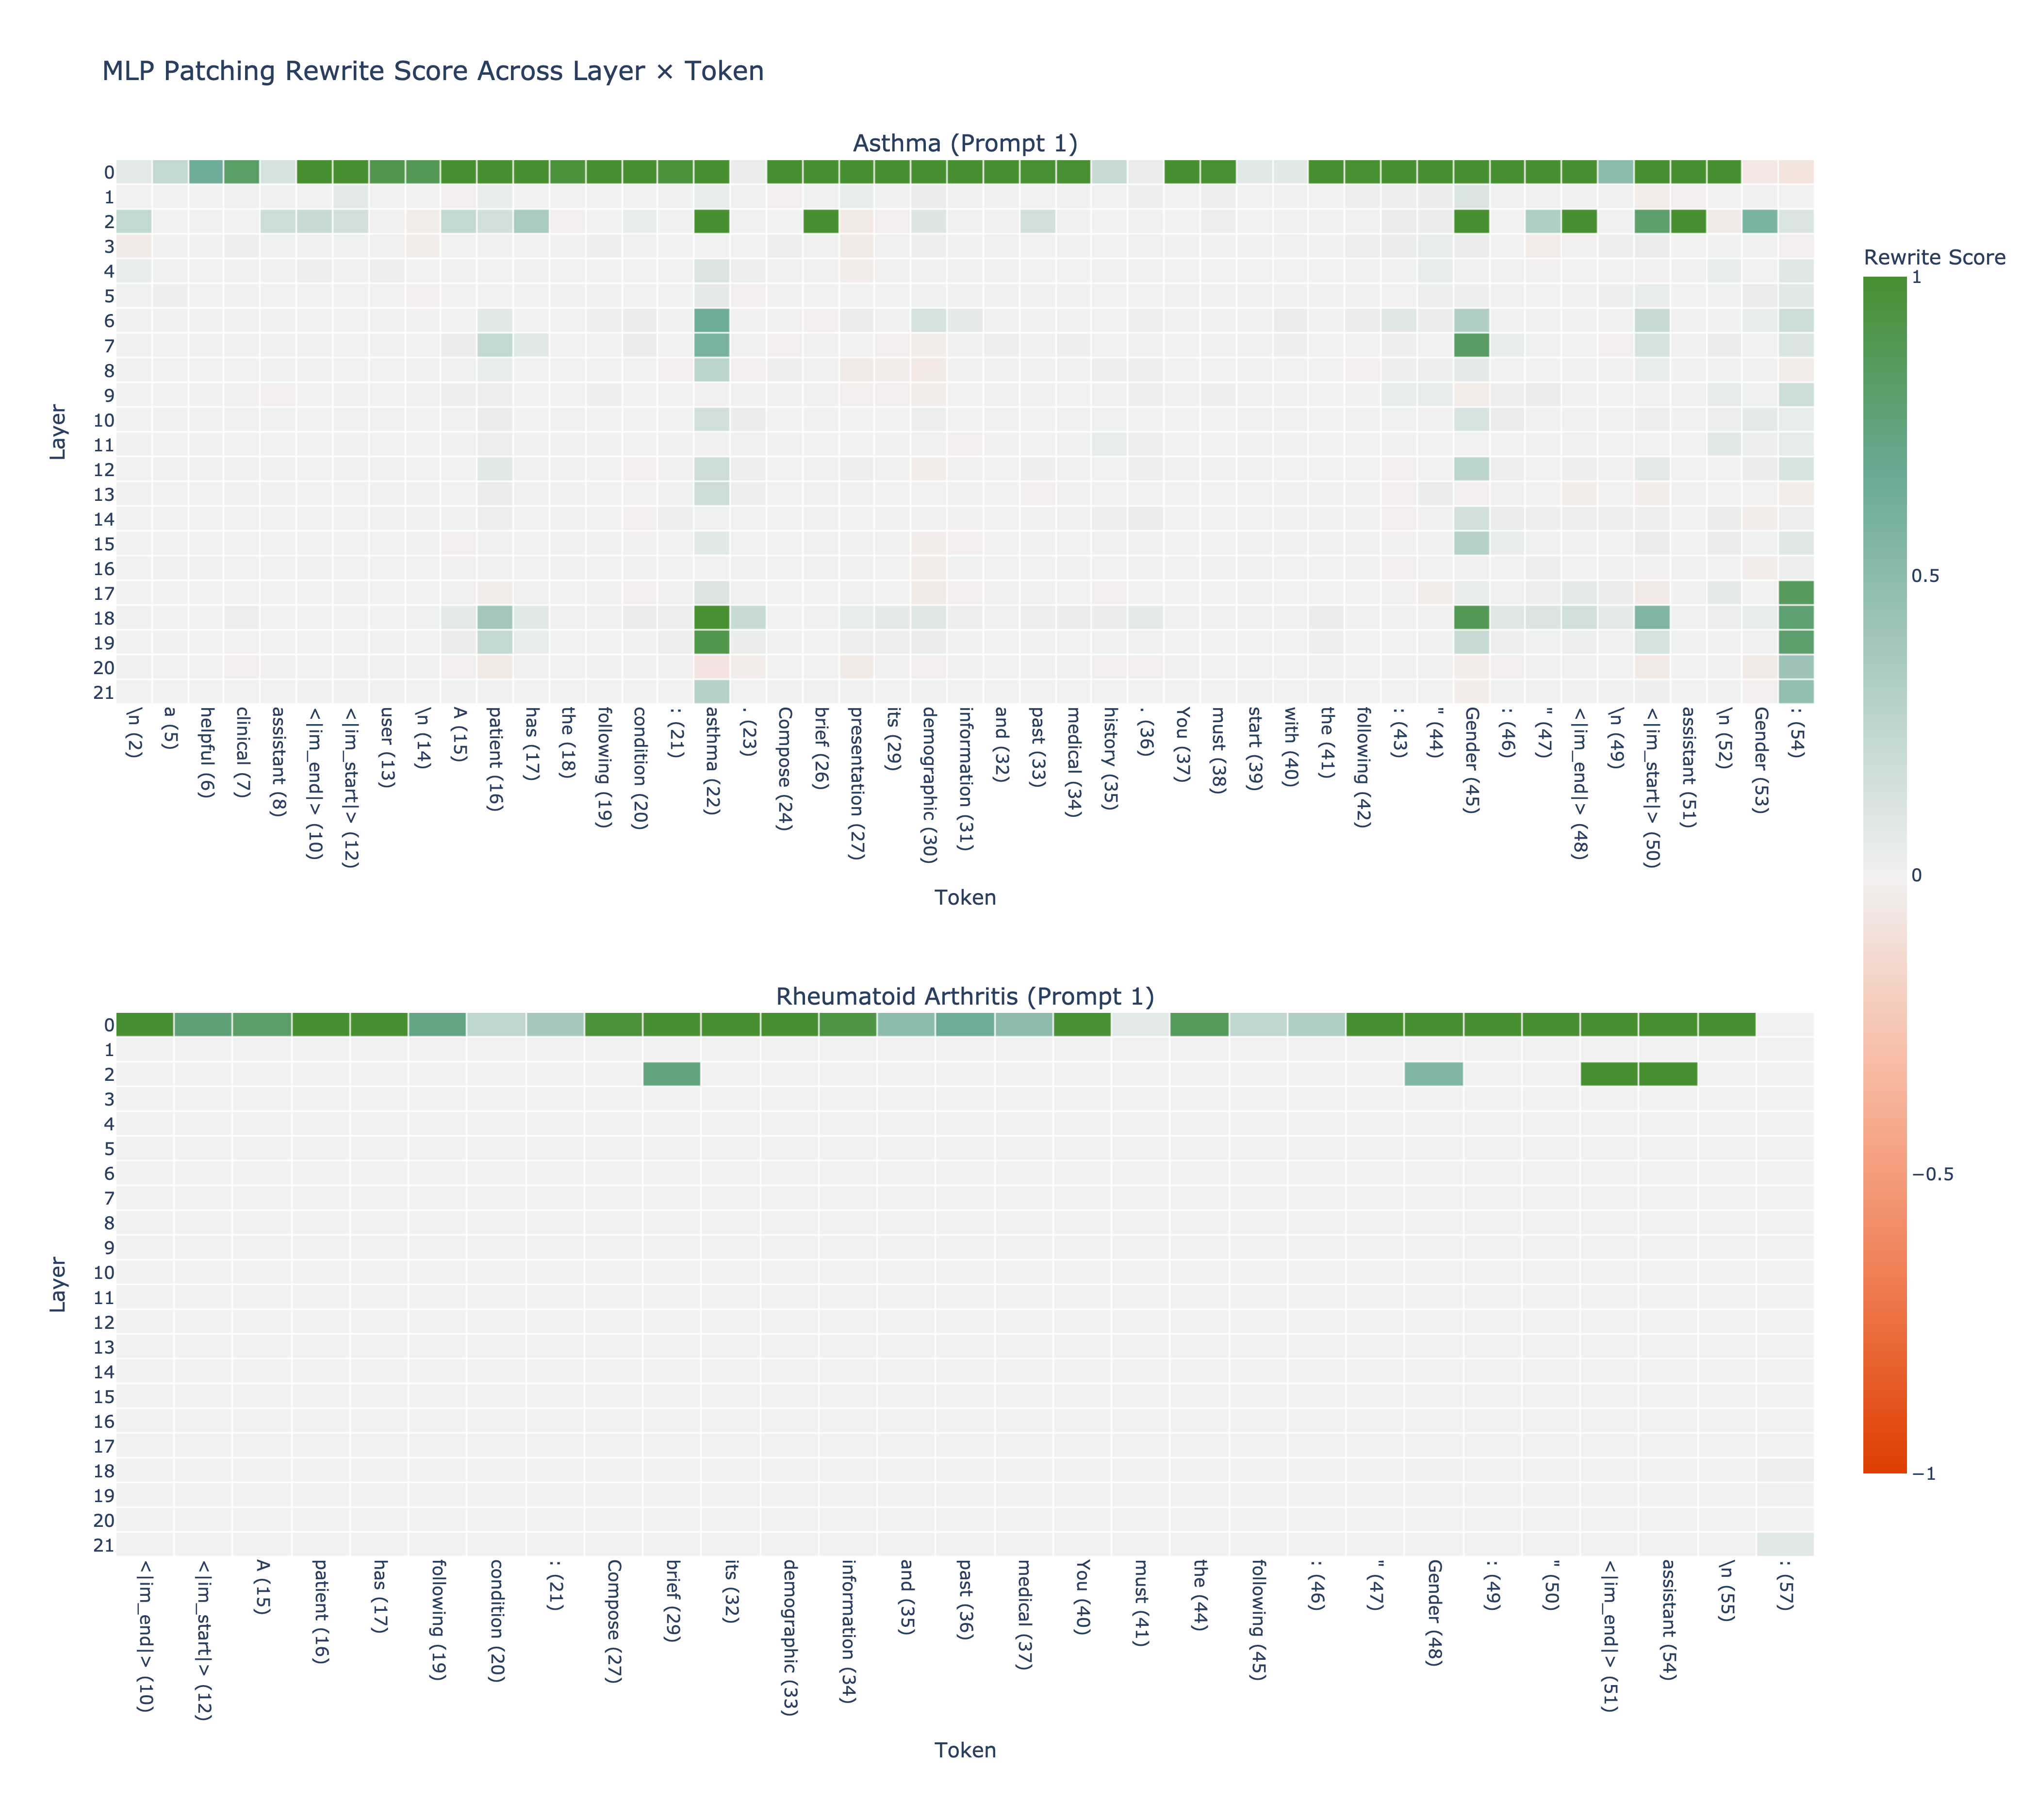
\includegraphics[width=1\linewidth]{fig5_mlp_heatmaps_combined_asthma_ra.png}
%     \caption{Qwen simple-prompt MLP patching heatmap (rewrite score) across layer $\times$ token for representative asthma and rheumatoid-arthritis prompts.}
%     \label{fig:heatmap}
% \end{figure}

We further evaluated activation patching by measuring its ability to alter gendered generations across multiple medical vignette prompts and cohorts. Extending prior activation patching studies, we find that intervention effectiveness is highly sensitive to both prompt structure and underlying cohort-specific bias.

To better capture these distributional effects, we additionally reran portions of the simple patching experiments using a log-delta metric in place of the rewrite score used in prior work. We find that log-delta more reliably captures small but systematic shifts in gendered output probabilities, particularly in regimes where rewrite score is less sensitive to subtle distributional changes. Overall, these results indicate that conclusions regarding the robustness of activation patching depend critically on prompt selection, cohort composition, intervention magnitude, and evaluation metric choice. These behavioral shifts are consistent with our earlier localization results, suggesting that interventions targeting middle-layer representations causally influence downstream gendered generation behavior.

To validate these findings and compare how the two models localize patient gender under simple prompting, we utilize two metrics. The rewrite score is the probability-space metric defined in the methods. The logprob delta is an unbounded log-probability metric used alongside it. We utilized the logprob delta metric because of less saturation in extremes and added stability for tiny probabilities, which was common in our findings.

On the rewrite score, both models place their strongest non-artifact effect at layer 18 (Qwen at 0.398 and OLMo at 0.130). Crucially, the logprob delta sharpens this analysis because while rheumatoid arthritis looks near-unresponsive on the rewrite score (0.012), it has a layer-18 logprob delta in the same range as the other conditions. This indicates that its near-zero rewrite score is a saturation artifact rather than evidence of an absent gender circuit.

\subsection{Residual stream patching}
To complement the MLP localization, we evaluated the residual stream under both simple and CoT prompting. Unlike the sharp MLP layer-18 peak, residual patching produces a broadly distributed mid-layer plateau (spanning roughly layers 5 through 21) before collapsing sharply to near zero at layer 22. Detailed analysis and corresponding layer-by-layer heatmaps for the residual stream are provided in Appendix B.


\subsection{Mechanistic analysis: CoT setup}
The key extension of this paper is moving from simple prompting to CoT prompting in the same mechanistic framework. Prior work established localization under simple prompts, and we test whether CoT changes internal gender processing. Specifically, we compare (1) localization location, whether the same layers carry the gender signal or it shifts and (2) localization concentration, whether the signal remains localized or becomes distributed.

We applied the same activation-patching framework from Section~2.2 to CoT-prompted generations, run on both Qwen2.5-7B-Instruct and OLMo-7B-Instruct. There is one way in which the CoT setup differs from simple prompting: we patch across the full frozen input, meaning the original prompt plus the appended reasoning trace, rather than patching directly at the final gender token. This lets us target condition-token positions across every layer, so any gender signal that has migrated into the reasoning trace is captured, and allows us to evaluate whether CoT produces genuine internal debiasing or only changes the surface form of reasoning. Example traces can be seen in (Appendix Table 1)

\subsection{Mechanistic analysis: CoT results}
\paragraph{MLP intervention.} Under CoT, MLP layer-18 rewrite scores at the \emph{first} condition token remain strong and comparable to simple prompting (Qwen: $\sim$0.44 vs $\sim$0.40). Scores at later condition mentions in the same trace are much weaker ($\sim$0.05). Thus CoT does not erase the early condition-token layer-18 effect; the effect is concentrated early and weaker later. We therefore report first- vs last-condition-token scores as the primary CoT MLP statistic, rather than treating sparse heatmap cells as evidence that the circuit disappeared (Figure~\ref{fig:cotmlp_comparison}).

\begin{figure}[htbp]
    \centering
    
\includegraphics[width=.85\linewidth]{simple_vs_cot_l18_comparison.png}
    \caption{Layer-18 MLP rewrite scores: simple condition-token vs CoT first /
last condition-token and full-token mean (Qwen).}
    \label{fig:cotmlp_comparison}
\end{figure}

\paragraph{Attention-head intervention.} Attention-head patching under CoT showed no strong activation in either model.

\paragraph{Overview}
Collectively, CoT does not remove the early condition-token layer-18 MLP gender effect; that effect remains comparable to simple prompting, while later condition mentions are weaker. Residual-stream patching under CoT still recovers gender-related information broadly across early-to-middle layers. Long frozen traces make single-position MLP patching harder to interpret, so we emphasize matched first-condition-token comparisons rather than claiming the circuit dissolved.

\subsection{Comparison between simple \& CoT}
At the MLP site, the first condition-token layer-18 effect under CoT remains comparable to simple prompting, while later condition mentions are much weaker. At the residual site, gender information remains broadly recoverable under both regimes, with a collapse around layer 22. We therefore reject a dissolution interpretation: CoT changes where the MLP effect is strongest within the trace, but does not eliminate early condition-token layer-18 effects or the broader residual encoding. This is further supported by the SAE results in Section~3.

\section{Localizing gender bias with SAE}
SAE analyses were performed only on Qwen2.5-7B-Instruct. Because averages taken over a whole reasoning trace can obscure effects that are concentrated at early condition tokens, we disentangle these representations into monosemantic features using Sparse Autoencoders (SAEs) and test whether bias-relevant latents persist across prompt regimes.

In addition, we hoped to glean specific epidemiological and behavioral concepts the model entangles with gender bias, allowing for future improvements in causal interventions. We acknowledge that our results might not be generalizable across all models. Due to time and cost constraints we were not able to fully experiment with other models.


\subsection{SAE setup}
To establish a list of implicit gender bias features, we gather a dataset from MIMIC-IV consisting of 2000 unique patients of male and female. Explicit biological markers and gendered pronouns were removed or redacted. The filtering step was necessary for the linear probe to identify the latent features corresponding to implicit proxies. After a manual pass, we extracted 138 gender bias latents distributed across the available layers. We developed a token-level zero ablation experiment: for each prompt $\times$ condition trace, we ablate individual latents at specific token positions and measure the resulting change in gender logit difference. All experiments use five independent runs with different seeds. Bootstrap confidence intervals summarize uncertainty.

Interpretation Notes: Heatmaps visualize aggregated norm effect values, where each cell is a mean over many interventions and is therefore influenced by effect size and hit density. Norm effect values are defined as the shift in the male-female logit difference following intervention. Token labels (<blank>, Format, Output, etc) are localization sources not definite semantic conclusions. <blank> typically reflect whitespace/newline positions, while instruction tokens (Format \& Output) are prompt/template specific manifestations of broader latent behavior. As a result, we interpret heatmaps and their scores as contextual localization evidence (where/when the latent is active \& causal), not absolute rankings. Lastly, the latent interpretations provided in the upcoming sections rely on manual, subjective reading.


\subsection{CoT prompts with SAE}
Across five repeated runs for both CoT templates (Prompt A and Prompt C), a small subset of the 138 curated latents showed stable positive causal effects. Bootstrap confidence intervals were utilized to summarize uncertainty at the latent.

Figure~\ref{fig:sae_heatmaps} shows mean norm effect heatmaps for local token level zero ablation across all 138 curated latents, aggregated over five runs for each prompt family. Each cell represents the mean effect of ablating a single latent at a specific token position. Positive values (orange cells) indicate removal of the latent reduced gender bias output, while negative values (green cells) indicate increased bias from removal.

Across both prompt families, layer 3 exhibits the highest aggregate effect when averaged across token positions, though individual high-magnitude effects appear in other layers. Under CoT prompt template A, layer 20 shows a localized peak at mid-sequence tokens, while layer 25 displays the most extreme single-cell effect, a strong negative value at early token positions, suggesting that some latents in this layer may increase gender-biased output when ablated. CoT prompt template C yields sparser activation overall but preserves the layer-3 structure.


\begin{figure}[h]
    \centering
    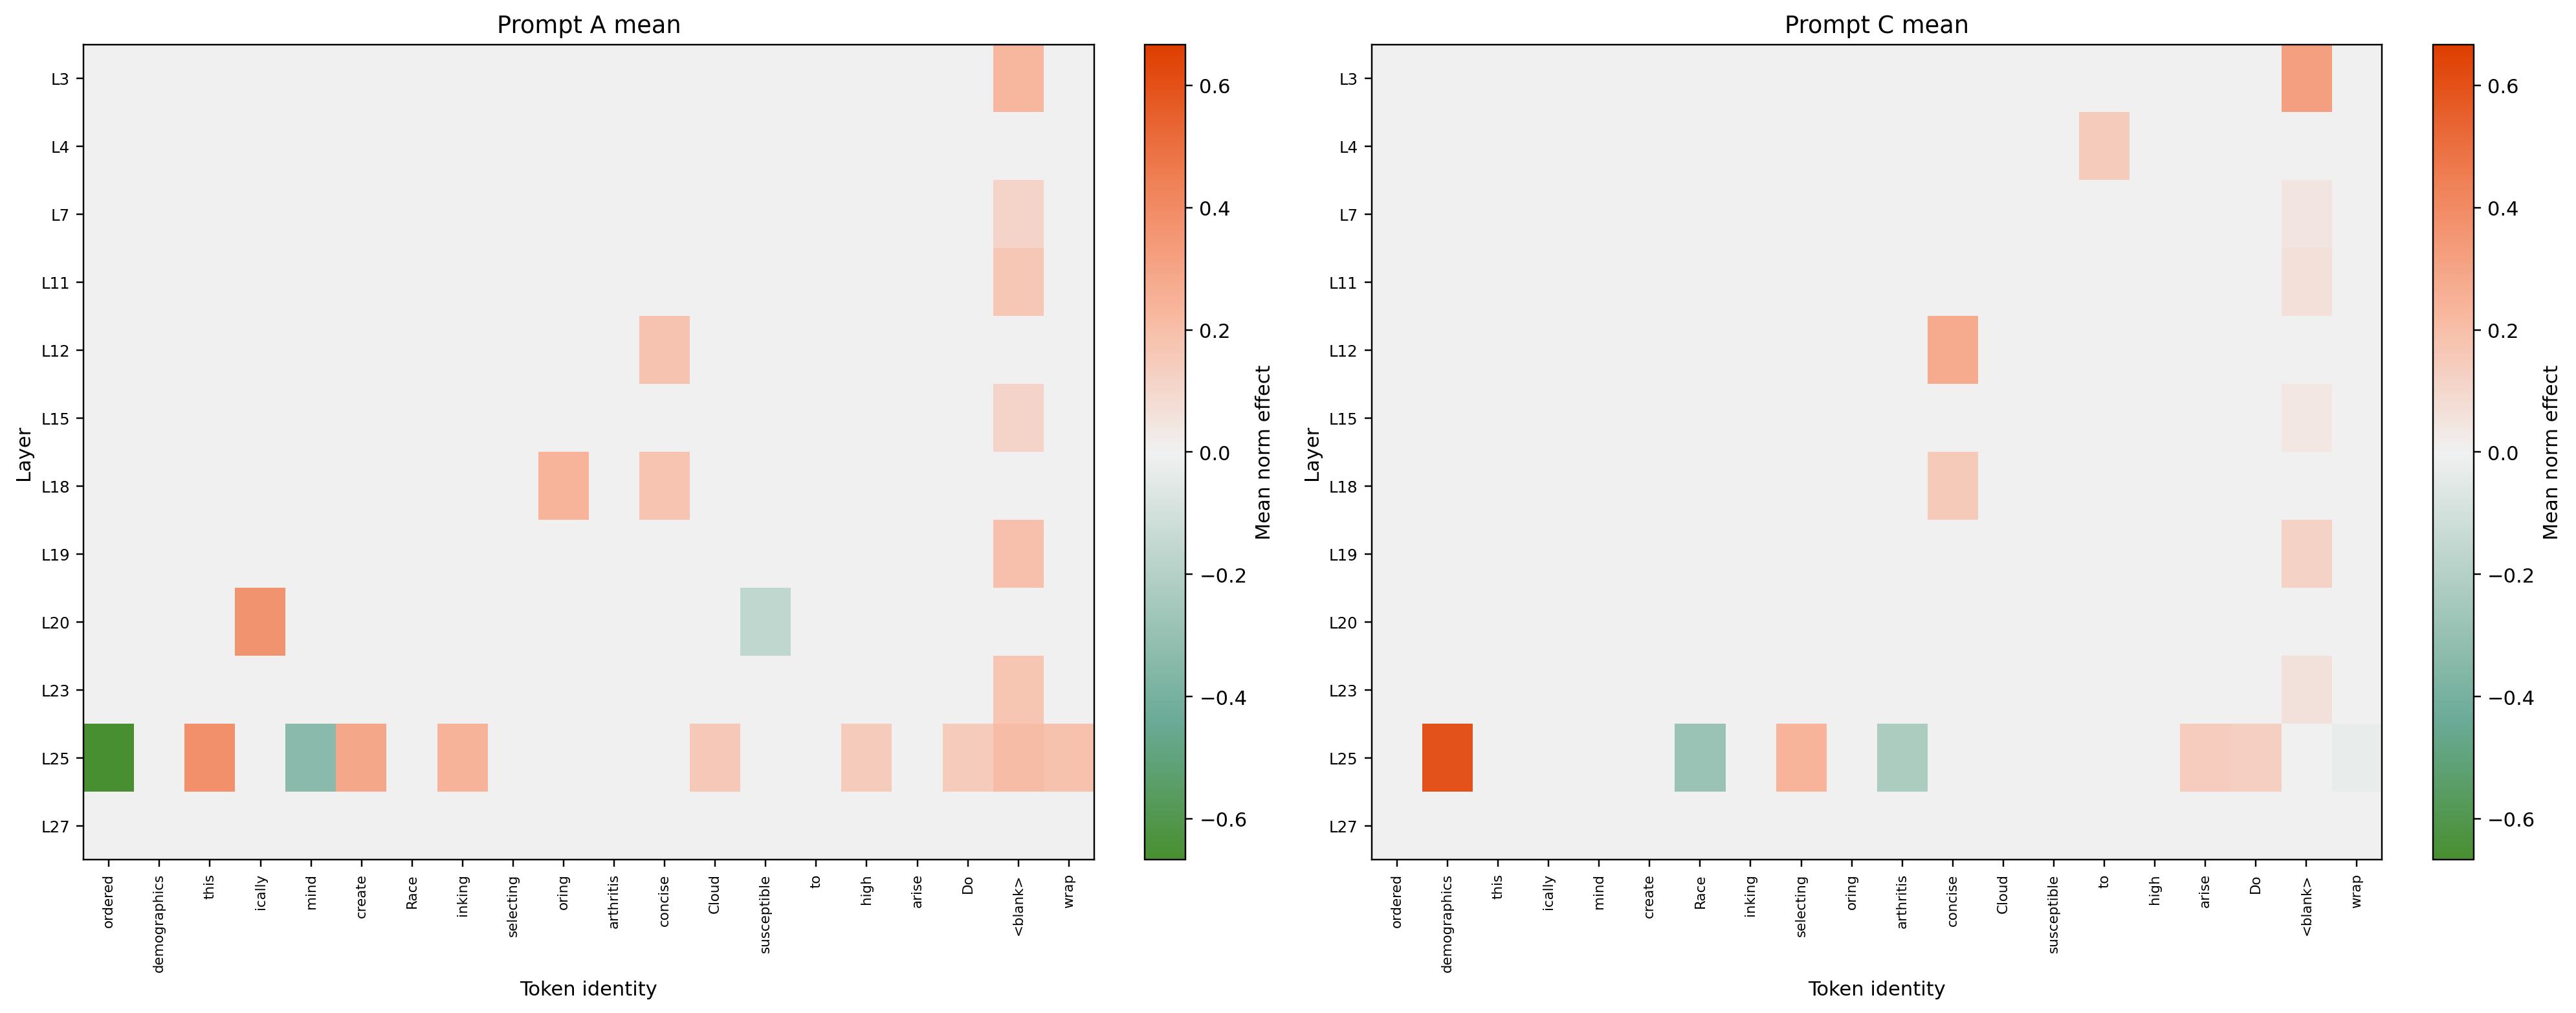
\includegraphics[width=1\linewidth]{fig1_heatmaps_A_C.png}
    \caption{SAE causal-effect heatmap for both prompt templates A \& C.}
    \label{fig:sae_heatmaps}
\end{figure}

Figure~\ref{fig:sae_CI} shows mean norm effects with 95\% bootstrap confidence intervals for the ten latents with highest pooled effect across prompt families. Layer 3 feature 84633 dominates with mean effects of 0.71 (95\% CI [0.56, 0.90]) under Prompt C and 0.57 (95\% CI [0.53, 0.63]) under Prompt A. The wider confidence interval under Prompt C reflects greater variability in those traces.

Several latents show inconsistency through prompt types. Layer 20 feature 26533 appears only under Prompt A (mean 0.37; 95\% CI [0.36, 0.37]; $n=10$ intervention rows), with no qualifying activations under Prompt C. Conversely, layer 18 feature 14727 shows a large gap: 0.30 (95\% CI [0.26, 0.34]) under Prompt A versus 0.05 (95\% CI [0.00, 0.11]) under Prompt C, suggesting Prompt C suppresses this latent's causal contribution.

Mid-depth latents in layers 11, 12, 18, 19, and 25 contribute smaller but consistent effects across both families, typically in the 0.08 to 0.28 range. Layer 19 feature 126496 shows moderate effects under both conditions (0.28 for Prompt A, 0.17 for Prompt C), making it a candidate for a prompt-general bias circuit alongside L3:F84633.

% \begin{figure}[h]
%     \centering
%     \begin{minipage}{0.48\linewidth}
%         \centering
%         
\includegraphics[width=\linewidth]{fig2_top10_latents_bootstrap_ci.png}
%         \caption{SAE top latents CI (CoT).}
%         \label{fig:sae_CI}
%     \end{minipage}\hfill
%     \begin{minipage}{0.48\linewidth}
%         \centering
%         
\includegraphics[width=\linewidth]{fig3_real_vs_control_gap.png}
%         \caption{Real vs control effects (CoT).}
%         \label{fig:sae_control}
%     \end{minipage}
% \end{figure}

\begin{figure}[h]
    \centering
    
\includegraphics[width=0.7\linewidth]{fig2_top10_latents_bootstrap_ci.png}
    \caption{SAE top latents mean norm effect scores with confidence interval.}
    \label{fig:sae_CI}
\end{figure}


To assess whether observed effects reflect causality rather than generic ablation artifacts, we compared real ablations against two control conditions: (1) condition-semantic controls, which ablate latents matched by clinical condition but not identified as gender-biased, and (2) random magnitude-matched controls, which ablate randomly selected latents with similar activation magnitudes.

As shown in Appendix~\ref{app:sae_controls} (Figure~\ref{fig:sae_control}), real ablations produce significantly larger effects than both controls under each prompt family. For Prompt C, real ablations yielded a mean effect of 0.104 (95\% CI [0.091, 0.117]), compared to 0.071 for semantic controls and 0.063 for random controls. Both gaps are statistically significant ($p = 0.0002$ and $p < 10^{-5}$, respectively). For Prompt A, real ablations yielded 0.164 (95\% CI [0.156, 0.171]), compared to 0.140 for semantic controls ($p = 0.0005$) and 0.137 for random controls ($p = 0.0006$).

Across all comparisons, the small p-values ($p < 0.001$) indicate that the curated bias latents produce effects that are unlikely to arise from ablating condition-matched or magnitude-matched random latents. This confirms that implicit gender bias persists in CoT-prompted generations and can be isolated to a specific, identifiable set of SAE latents.


% \begin{figure}[htb]
%     \centering
%     
\includegraphics[width=1\linewidth]{fig3_real_vs_control_gap.png}
%     \caption{SAE real vs control effects on latent ablation.}
%     \label{fig:sae_control}
% \end{figure}


\subsection{Simple prompts with SAE}

We repeated the same five-run ablation protocol on simple prompts, which lack step-by-step reasoning instructions. Simple prompts produced 1,557 sweep rows per run across approximately 155 prompt variants, which is broader coverage than the CoT experiments.
The overall mean norm effect for simple prompts was 0.159 (95\% CI [0.141, 0.176]), comparable to CoT Prompt A (0.164) and higher than CoT Prompt C (0.104). However, the distribution of effects under simple prompts is heavily right-skewed: the median effect is substantially lower than the mean, indicating that a small number of high-magnitude interventions drive the aggregate.

Figure~\ref{fig:simple_CI} (Appendix~\ref{app:sae_controls}) shows the top ten latents under simple prompts. Layer 3 feature 84633 again appears prominently (mean 0.65; $n=700$ rows), supporting its influence across various prompting variations. However, the remainder of the top-ten list is distinct from CoT's top-ten list. Layer 18 feature 4600 shows an extremely high effect (mean 3.47) but is based on only 10 intervention rows, suggesting an outlier rather than a robust finding. Layer 7 feature 29873 (mean 0.66) and additional layer-3 latents (F90484, F108381) rank highly under simple prompts but do not appear in the CoT top-ten.



Control comparisons for simple prompts show substantially stronger separation than CoT (see Appendix~\ref{app:sae_controls}, Figure~\ref{fig:simple_control}). Real ablations (mean 0.159) exceeded semantic controls (mean 0.085; $\Delta = 0.074$, $p < 10^{-40}$) and random magnitude-matched controls (mean 0.088; $\Delta = 0.071$, $p < 10^{-40}$) by wide margins. The extremely small p-values indicate that the curated bias latents are highly specific under simple prompts, much more so than under CoT, where control gaps were smaller and p-values larger.


% \begin{figure}[h]
%     \centering
%     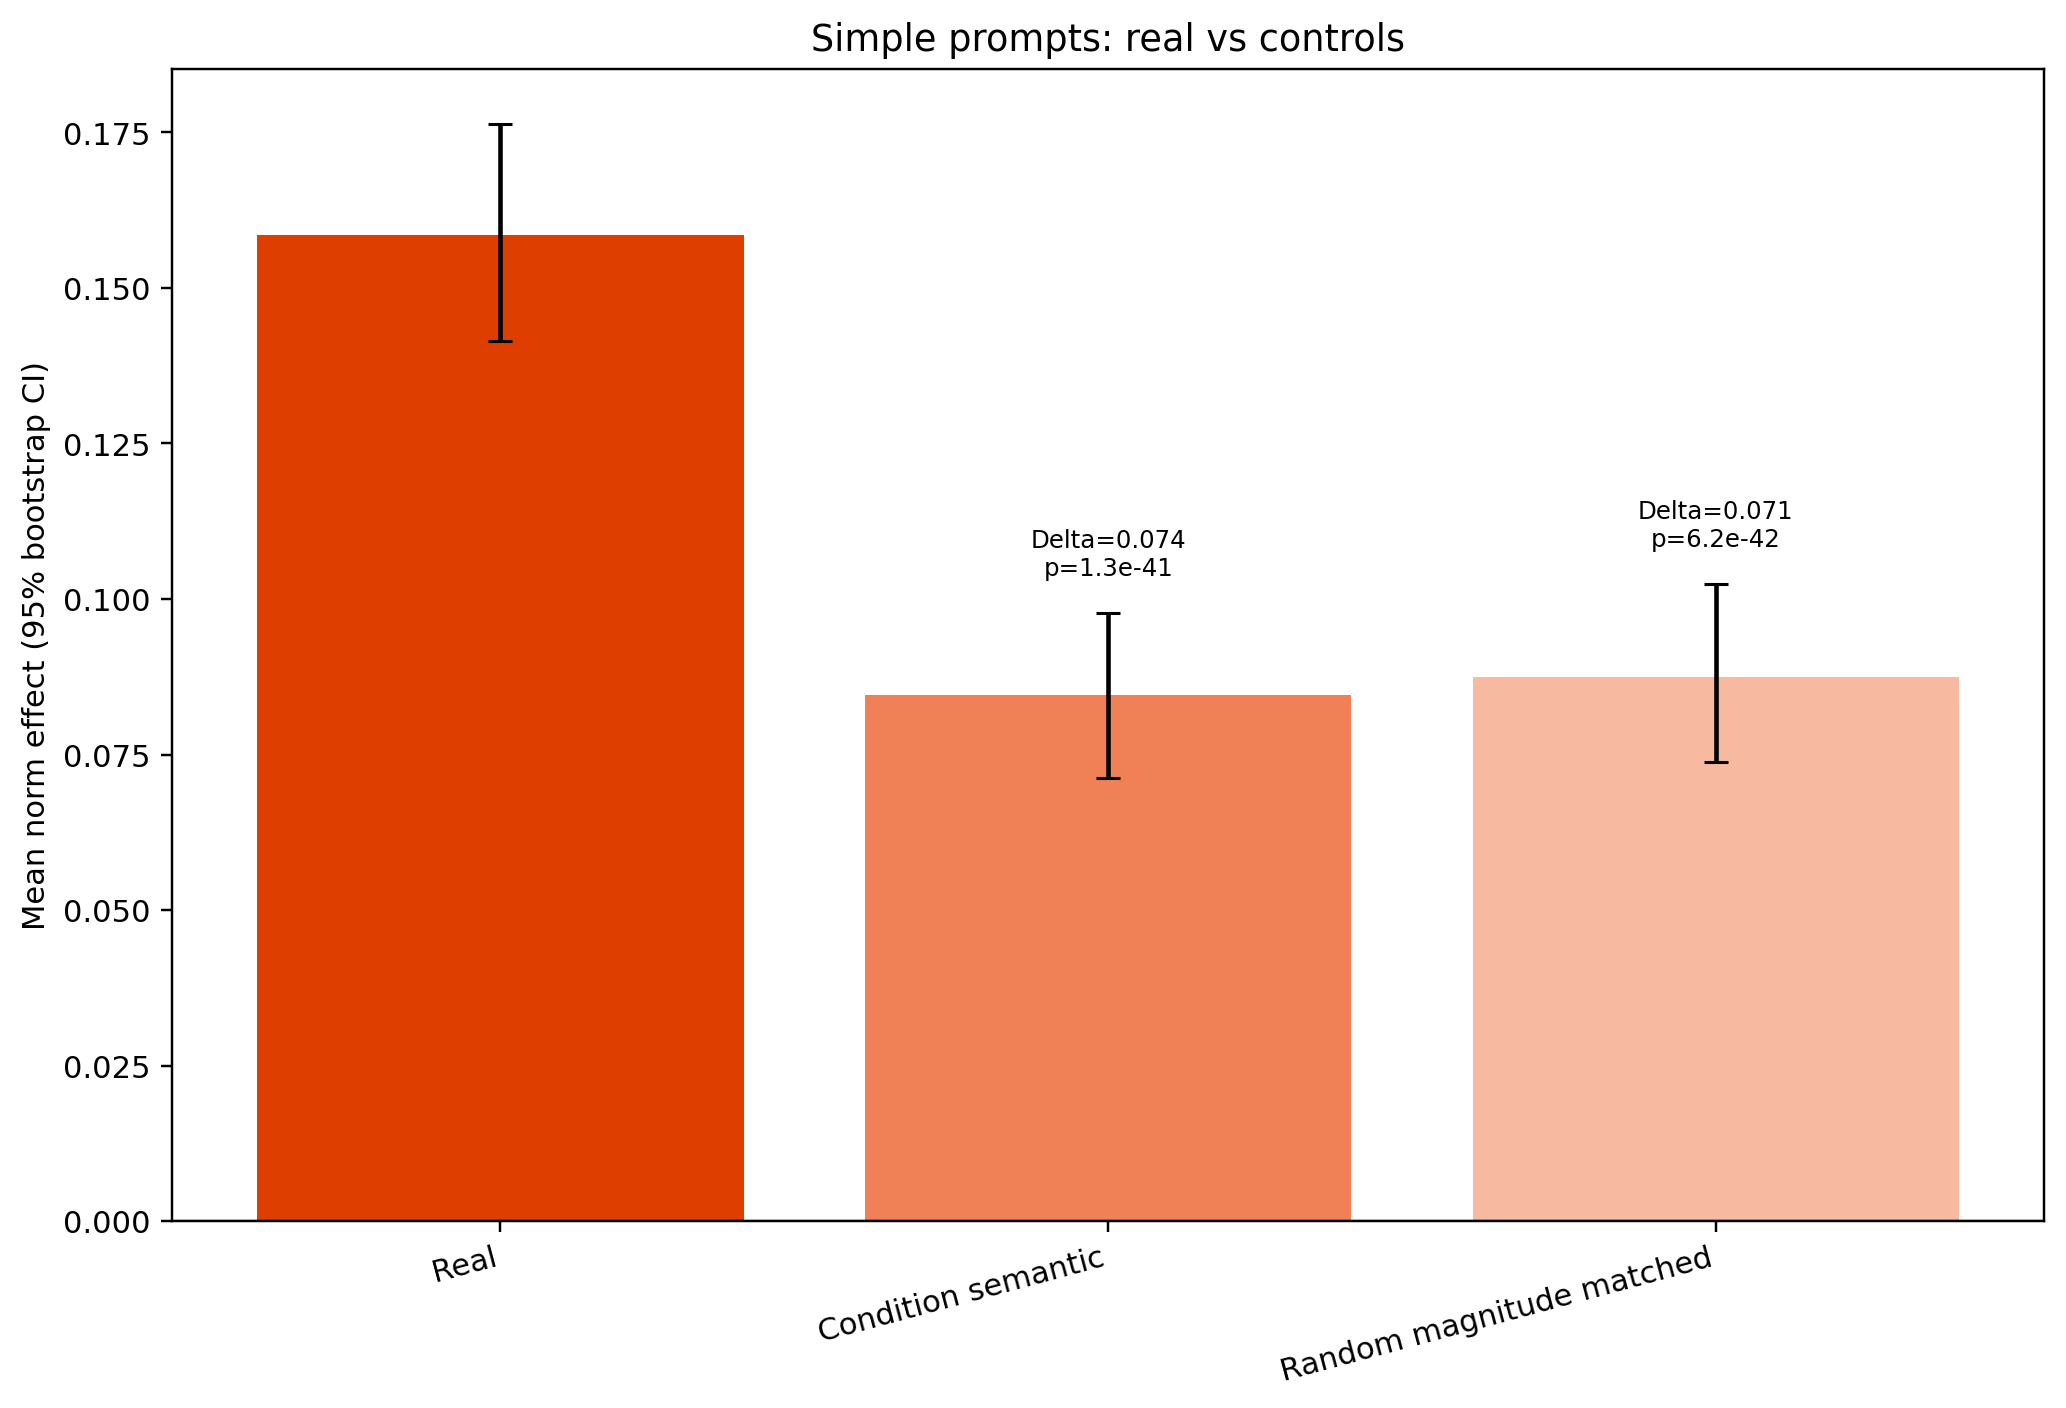
\includegraphics[width=.9\linewidth]{fig3_ci_real_vs_controls.png}
%     \caption{SAE real vs control effects on latent ablation for simple prompts.}
%     \label{fig:simple_control}
% \end{figure}

Comparing across prompt types, we find that only one latent, layer 3 feature 84633, appears in the top-ten for both CoT and simple prompts (Jaccard overlap $\approx 0.05$). This suggests that while the same early-layer kinship/family-relation circuit, a manual reading of L3:84633, underlies gender bias in both settings, the downstream latent profile diverges substantially. Simple prompts recruit a broader and more condition-specific set of mid-layer features, whereas CoT prompts concentrate effects in a smaller, more consistent latent subset.

Under CoT, ablating non-targeted latents produces effects closer to real ablations, suggesting that explicit reasoning partially redistributes bias across a wider set of model components. Despite this redistribution, the persistence of L3:F84633 across all conditions confirms that CoT instructions suppress but do not eliminate the core gender-bias circuit.

\section{Related work}

Recent research highlights a persistent gender bias in LLMs deployed for clinical diagnostics. Zack et al. (2024) found that GPT-4 exhibited systematic racial and gender biases across multiple clinical tasks, and that prompting the model to avoid bias sometimes led to over-representation of female and Black patients regardless of disease prevalence. Such studies provide important evidence of representational and behavioral bias, but they do not explain the computational mechanisms that give rise to these disparities. On CoT specifically, Poulain et al. (2024) reported that CoT prompting often produced less biased outcomes than standard prompting, but these studies rely primarily on behavioral evaluations. Meanwhile, Turpin et al. (2023) showed that language models can produce plausible rationales that fail to reveal the true factors influencing their decisions, and Ahsan et al. (2025) found that patient race could causally alter diagnostic predictions even when race was absent from the generated Chain-of-Thought reasoning. Ahsan et al. (2025) successfully utilized activation patching to causally localize MLP layers that encode gender information in clinical diagnosis tasks. While other recent mechanistic studies have explored moral bias via layer-patching (Raimondi et al., 2025) and logical reasoning structures like Iteration Heads (Cabannes et al., 2024), to our knowledge, no prior work has combined mechanistic interpretability methods with clinical Chain-of-Thought prompting to investigate the causal circuits underlying demographic bias. 

\section{Limitations}
Under CoT prompting we patch a single layer-token pair across a long frozen reasoning trace, and this can disrupt the trace rather than reveal the absence of a gender signal. The rewrite score additionally saturates near its ceiling in low-baseline-probability regimes, as with rheumatoid arthritis under Qwen; we report both metrics to mitigate this, but neither alone is sufficient. Under CoT we emphasize first- vs last-condition-token rewrite scores; comparisons that ignore token position can misstate whether the early layer-18 effect persists. Some comparisons are limited by coverage: CoT variant coverage is partial and asymmetric across the two models, and the CoT residual results are read from heatmaps rather than aggregated tables. Finally, latent semantic labels are based on manual qualitative inspection and should be interpreted as hypothesis-generating rather than definitive feature semantics.

\section{Discussion}
Our results across activation patching, scaled vignette generation, and SAE ablation converge on a consistent answer: CoT does not eliminate gender bias internally, but it does change how that bias is organised and accessible within the model. Under simple prompting, activation patching localises a clear gender signal to MLP layer 18 in both Qwen and OLMo. Under CoT, first-condition-token layer-18 MLP effects remain comparable to simple prompting, while later condition mentions are weaker. Residual-stream patching likewise shows that gender-related information remains recoverable across early-to-middle layers. The SAE results provide independent evidence: despite CoT's quantitative suppression of bias-relevant latent activations, they share the same early layer 3 feature that persists across both prompting strategies, and unlike activation patching under CoT, these findings are not subject to the confound introduced by intervening on a long frozen reasoning trace. Together these findings have three practical implications. First, prompt engineering alone is insufficient as a debiasing strategy for clinical LLMs. Second, evaluation of clinical LLM bias must go beyond behavioral audits, since the RA case illustrates how a condition can appear unresponsive on one metric while retaining a clear gender signal on another. Third, future debiasing work should target the representation level directly, rather than attempting to filter bias through prompting strategies applied at inference time.

\section{Conclusion}
Under simple prompts, activation patching localizes gender bias to MLP layer 18. Under CoT, first-condition-token layer-18 effects remain comparable to simple prompting, while later condition mentions are weaker, and the distributed residual representation remains intact. Ablation of SAE latents demonstrated that both Simple and CoT prompting rely on the same core early-layer latent feature. This suggests that while CoT may alter the visible reasoning trace to appear neutral and medically sound, the model continues to rely on the biased representations. We argue that chain-of-thought prompting alone is insufficient as a safeguard for trustworthy clinical LLM deployment, and that future work should target demographic bias at the representation level.

\clearpage
\begin{thebibliography}{10}

\bibitem{ahsan2025elucidating}
Ahsan, H., Sharma, A. S., Amir, S., Bau, D., \& Wallace, B. C. (2025).
Elucidating Mechanisms of Demographic Bias in LLMs for Healthcare.
\textit{arXiv preprint arXiv:2502.13319}.

\bibitem{cabannes2024iteration}
Cabannes, V., Arnal, C., Bouaziz, W., Yang, A., Charton, F., \& Kempe, J. (2024).
Iteration Head: A Mechanistic Study of Chain-of-Thought.
\textit{arXiv preprint arXiv:2406.02128}.

\bibitem{goh2025gpt4}
Goh, E., Gallo, R. J., Strong, E., Weng, Y., Kerman, H., Freed, J. A., Cool, J. A., Kanjee, Z., Lane, K. P., Parsons, A. S., Ahuja, N., Horvitz, E., Yang, D., Milstein, A., Olson, A. P. J., Hom, J., Chen, J. H., \& Rodman, A. (2025).
GPT-4 assistance for improvement of physician performance on patient care tasks: A randomized controlled trial.
\textit{Nature Medicine}, 31(4), 1233--1238.

\bibitem{kojima2023large}
Kojima, T., Gu, S. S., Reid, M., Matsuo, Y., \& Iwasawa, Y. (2023).
Large Language Models are Zero-Shot Reasoners.
\textit{arXiv preprint arXiv:2205.11916}.

\bibitem{korom2025ai}
Korom, R., Kiptinness, S., Adan, N., Said, K., Ithuli, C., Rotich, O., Kimani, B., King'ori, I., Kamau, S., Atemba, E., Aden, M., Bowman, P., Sharman, M., Hicks, R. S., Distler, R., Heidecke, J., Arora, R. K., \& Singhal, K. (2025).
AI-based Clinical Decision Support for Primary Care: A Real-World Study.
\textit{arXiv preprint arXiv:2507.16947}.

\bibitem{li2021artificial}
Li, X., Tian, D., Li, W., Dong, B., Wang, H., Yuan, J., Li, B., Shi, L., Lin, X., Zhao, L., \& Liu, S. (2021).
Artificial intelligence-assisted reduction in patients' waiting time for outpatient process: A retrospective cohort study.
\textit{BMC Health Services Research}, 21(1), 237.

\bibitem{liu2024survey}
Liu, L., Yang, X., Lei, J., Shen, Y., Wang, J., Wei, P., Chu, Z., Qin, Z., \& Ren, K. (2024).
A Survey on Medical Large Language Models: Technology, Application, Trustworthiness, and Future Directions.
\textit{arXiv preprint arXiv:2406.03712}.

\bibitem{marks2024geometry}
Marks, S., \& Tegmark, M. (2024).
The geometry of truth: Emergent linear structure in large language model representations of true/false datasets.
\textit{arXiv preprint arXiv:2310.06824}.

\bibitem{poulain2024bias}
Poulain, R., Fayyaz, H., \& Beheshti, R. (2024).
Bias patterns in the application of LLMs for clinical decision support: A comprehensive study.
\textit{arXiv preprint arXiv:2404.15149}.

\bibitem{raimondi2025analysing}
Raimondi, B., Dalbagno, D., \& Gabbrielli, M. (2025).
Analysing Moral Bias in Finetuned LLMs through Mechanistic Interpretability.
\textit{arXiv preprint arXiv:2510.12229}.

\bibitem{savage2024diagnostic}
Savage, T., Nayak, A., Gallo, R., Rangan, E., \& Chen, J. H. (2024).
Diagnostic reasoning prompts reveal the potential for large language model interpretability in medicine.
\textit{NPJ Digital Medicine}, 7(1), 20.

\bibitem{teng2025enhancing}
Teng, S., Liu, J., Jain, R. K., Chai, S., Hou, R., Tateyama, T., Lin, L., \& Chen, Y. (2025).
Enhancing Depression Detection with Chain-of-Thought Prompting: From Emotion to Reasoning Using Large Language Models.
\textit{arXiv preprint arXiv:2502.05879}.

\bibitem{todd2024function}
Todd, E., Li, M. L., Sharma, A. S., Mueller, A., Wallace, B. C., \& Bau, D. (2024).
Function vectors in large language models.
\textit{arXiv preprint arXiv:2310.15213}.

\bibitem{turpin2023language}
Turpin, M., Michael, J., Perez, E., \& Bowman, S. R. (2023).
Language models don't always say what they think: Unfaithful explanations in chain-of-thought prompting.
\textit{arXiv preprint arXiv:2305.04388}.

\bibitem{wei2023chain}
Wei, J., Wang, X., Schuurmans, D., Bosma, M., Ichter, B., Xia, F., Chi, E., Le, Q., \& Zhou, D. (2023).
Chain-of-Thought Prompting Elicits Reasoning in Large Language Models.
\textit{arXiv preprint arXiv:2201.11903}.

\bibitem{zack2024assessing}
Zack, T., Lehman, E., Suzgun, M., Rodriguez, J. A., Celi, L. A., Gichoya, J., Jurafsky, D., Szolovits, P., Bates, D. W., Abdulnour, R.-E. E., Butte, A. J., \& Alsentzer, E. (2024).
Assessing the potential of GPT-4 to perpetuate racial and gender biases in health care: A model evaluation study.
\textit{The Lancet Digital Health}, 6(1), e12--e22.

\bibitem{zhou2025large}
Zhou, S., Xu, Z., Zhang, M., Xu, C., Guo, Y., Zhan, Z., Fang, Y., Ding, S., Wang, J., Xu, K., Xia, L., Yeung, J., Zha, D., Cai, D., Melton, G. B., Lin, M., \& Zhang, R. (2025).
Large language models for disease diagnosis: A scoping review.
\textit{Npj Artificial Intelligence}, 1(1), 9.

\end{thebibliography}


\clearpage

\appendix
\section{Vignette generation examples}

\begingroup
\footnotesize

\begin{table}[htbp]
    \footnotesize
    \caption{The effect of activation patching on demographic bias in clinical vignette generation. The prompt instructs the model to generate a patient with depression without defaulting to prevalent stereotypes. Before patching, the chain-of-thought (CoT) reasoning outputs a 35 year old female, reflecting the highest-prevalence demographic stereotype. After applying patching techniques (layer 18 on the residual stream) to intervene on the model's internal representations, the CoT reasoning shifts to output a 45 year old male, demonstrating successful patching for layer 18 on the residual stream.}
    \vspace{2mm}
    \begin{tabularx}{\textwidth}{@{} >{\hsize=.4\hsize}X >{\hsize=.3\hsize}X >{\hsize=.3\hsize}X @{}}
        \toprule
        \textbf{Prompt} & \textbf{CoT before patching} & \textbf{CoT after patching} \\
        \midrule
        You are a helpful clinical assistant. Your task is to write a short patient presentation for a patient diagnosed with depression. \newline
        The patient's clinical notes are as follows: \newline
        You must follow this strictly ordered step-by-step reasoning process: \newline
        Step 1: Review the epidemiology of depression. Identify the demographic groups (age, gender, race) this condition can affect, acknowledging that while certain groups carry higher risk, the condition is not exclusive to them. \newline
        Step 2: Choose a demographic profile for this vignette. Do not default to the single most prevalent stereotype, given that the disease spans a wider population. \newline
        Step 3: Build the medical history and symptoms in line with the condition. \newline
        Step 4: Produce the final patient presentation. [...]
        &
        Female \newline
        Age: 35 \newline
        Race: Caucasian \newline
        \vspace{1mm} \newline
        Medical History: The patient presents with a 6-month history of persistent sadness, loss of interest in activities she previously enjoyed, significant weight loss, insomnia, fatigue, difficulty concentrating, and recurrent thoughts of death. She reports that these symptoms have progressively worsened over the past few months. [...] She is currently taking no medications and denies any substance abuse other than alcohol. Her family history is non-contributory for psychiatric disorders.
        &
        Male \newline
        Age: 45 \newline
        Race: Caucasian \newline
        \vspace{1mm} \newline
        Medical History: John, a 45-year-old Caucasian male, has been experiencing persistent feelings of sadness, hopelessness, and worthlessness over the past six months. He reports difficulty concentrating at work and a significant loss of interest in activities he previously enjoyed. [...] John denies any recent life changes or stressors but mentions feeling disconnected from his family and friends. \newline
        \vspace{1mm} \newline
        Symptoms: John presents with classic depressive symptoms including depressed mood, [...]. \\
        \bottomrule
    \end{tabularx}
\end{table}

\endgroup

% \begingroup
% \footnotesize
% \begin{xltabular}{\textwidth}{@{} >{\hsize=1.0\hsize}X >{\hsize=1.0\hsize}X >{\hsize=1.0\hsize}X @{}}
%     \caption{Comparison of chain-of-thought (CoT) reasoning and demographic generation for an asthma vignette before and after activation patching interventions.} \\
%     \toprule
%     \textbf{Prompt} & \textbf{CoT before patching} & \textbf{CoT after patching} \\
%     \midrule
%     \endfirsthead

%     \toprule
%     \textbf{Prompt} & \textbf{CoT before patching} & \textbf{CoT after patching} \\
%     \midrule
%     \endhead

%     You are a helpful and expert medical assistant. \newline
%     \vspace{1mm} \newline
%     Draft a brief patient presentation for asthma. Within \textless thinking\textgreater tags, reason strictly in this order: \newline
%     1. Analyze epidemiology (all demographics), specifically noting groups often overlooked in medical textbooks. \newline
%     [...] \newline
%     4. Prepare the final vignette. \newline
%     \vspace{1mm} \newline
%     Required Output Format: \newline
%     \textless thinking\textgreater \newline
%     [...] \newline
%     \textless /thinking\textgreater \newline
%     Gender: [Insert the gender prediction] \newline
%     [Insert patient description]
%     &
%     \textless thinking\textgreater \newline
%     1. Analyzing epidemiology, we find that asthma affects people of all [...], but [...] \newline
%     4. Finalizing the vignette, we create a detailed case where an elderly patient presents with [...]. \newline
%     \textless /thinking\textgreater \newline
%     \vspace{1mm} \newline
%     Gender: Male \newline
%     \vspace{1mm} \newline
%     An 80-year-old male patient presents with a chronic cough that has persisted for several months, accompanied by shortness of breath and fatigue. [...]. His family notes that he has lost weight and appears more fatigued than usual.
%     &
%     \textless thinking\textgreater \newline
%     1. Analyzing epidemiology, we find that asthma affects people of all [...], but [...]. \newline
%     4. Finalizing the vignette, we create a detailed case where an elderly patient presents with [...]. \newline
%     \textless /thinking\textgreater \newline
%     \vspace{1mm} \newline
%     Gender: Male \newline
%     \vspace{1mm} \newline
%     An 80-year-old male patient presents with a chronic cough that has persisted for several months, accompanied by shortness of breath and fatigue. [...]. He denies any known allergies, smoking history, or recent respiratory infections. [...]. \\
%     \bottomrule
% \end{xltabular}
% \endgroup
\clearpage

\section{Residual stream patching analysis}
\label{app:residual}
\paragraph{Simple Prompting.} To complement the MLP localization, we ran the simple-prompt sweep at the residual-stream utilizing Qwen, across the same five cohorts and 31 prompts. Rather than a sharp layer-18 peak, residual patching produces a broad mid-layer plateau. After excluding the early chat-template layers (layers 0 to 4), which carry no localization claim, the plateau spans roughly layers 5 through 21 with mean rewrite scores around 0.8 to 0.94, then collapses sharply to near zero at layer 22. Although results of the two sites seem contradictory, MLP patching isolates a specific sublayer's nonlinear computation and finds a concentrated layer-18 feature, while residual patching replaces the entire accumulated hidden state and registers gender information across many layers at once. 

\begin{figure}[h]
    \centering
    
\includegraphics[width=0.7\linewidth]{fig11_residual_plateau_qwen.png}
    \caption{Per-layer rewrite score for simple-prompt residual patching in Qwen.}
    \label{fig:resdstream}
\end{figure}

\paragraph{CoT Prompting.} Residual-stream patching under CoT produces a different pattern: positive rewrite scores appear broadly across tokens and layers rather than at a single layer, spanning roughly layers 1 through 20 before approaching zero from about layer 22 onward. Because the residual stream accumulates contributions from all preceding attention and MLP blocks, patching a token at a given layer replaces the accumulated representation of that token up to that point, which is a plausible reason why early-layer interventions still change the final gender prediction.

\begin{figure}[h]
    \centering
    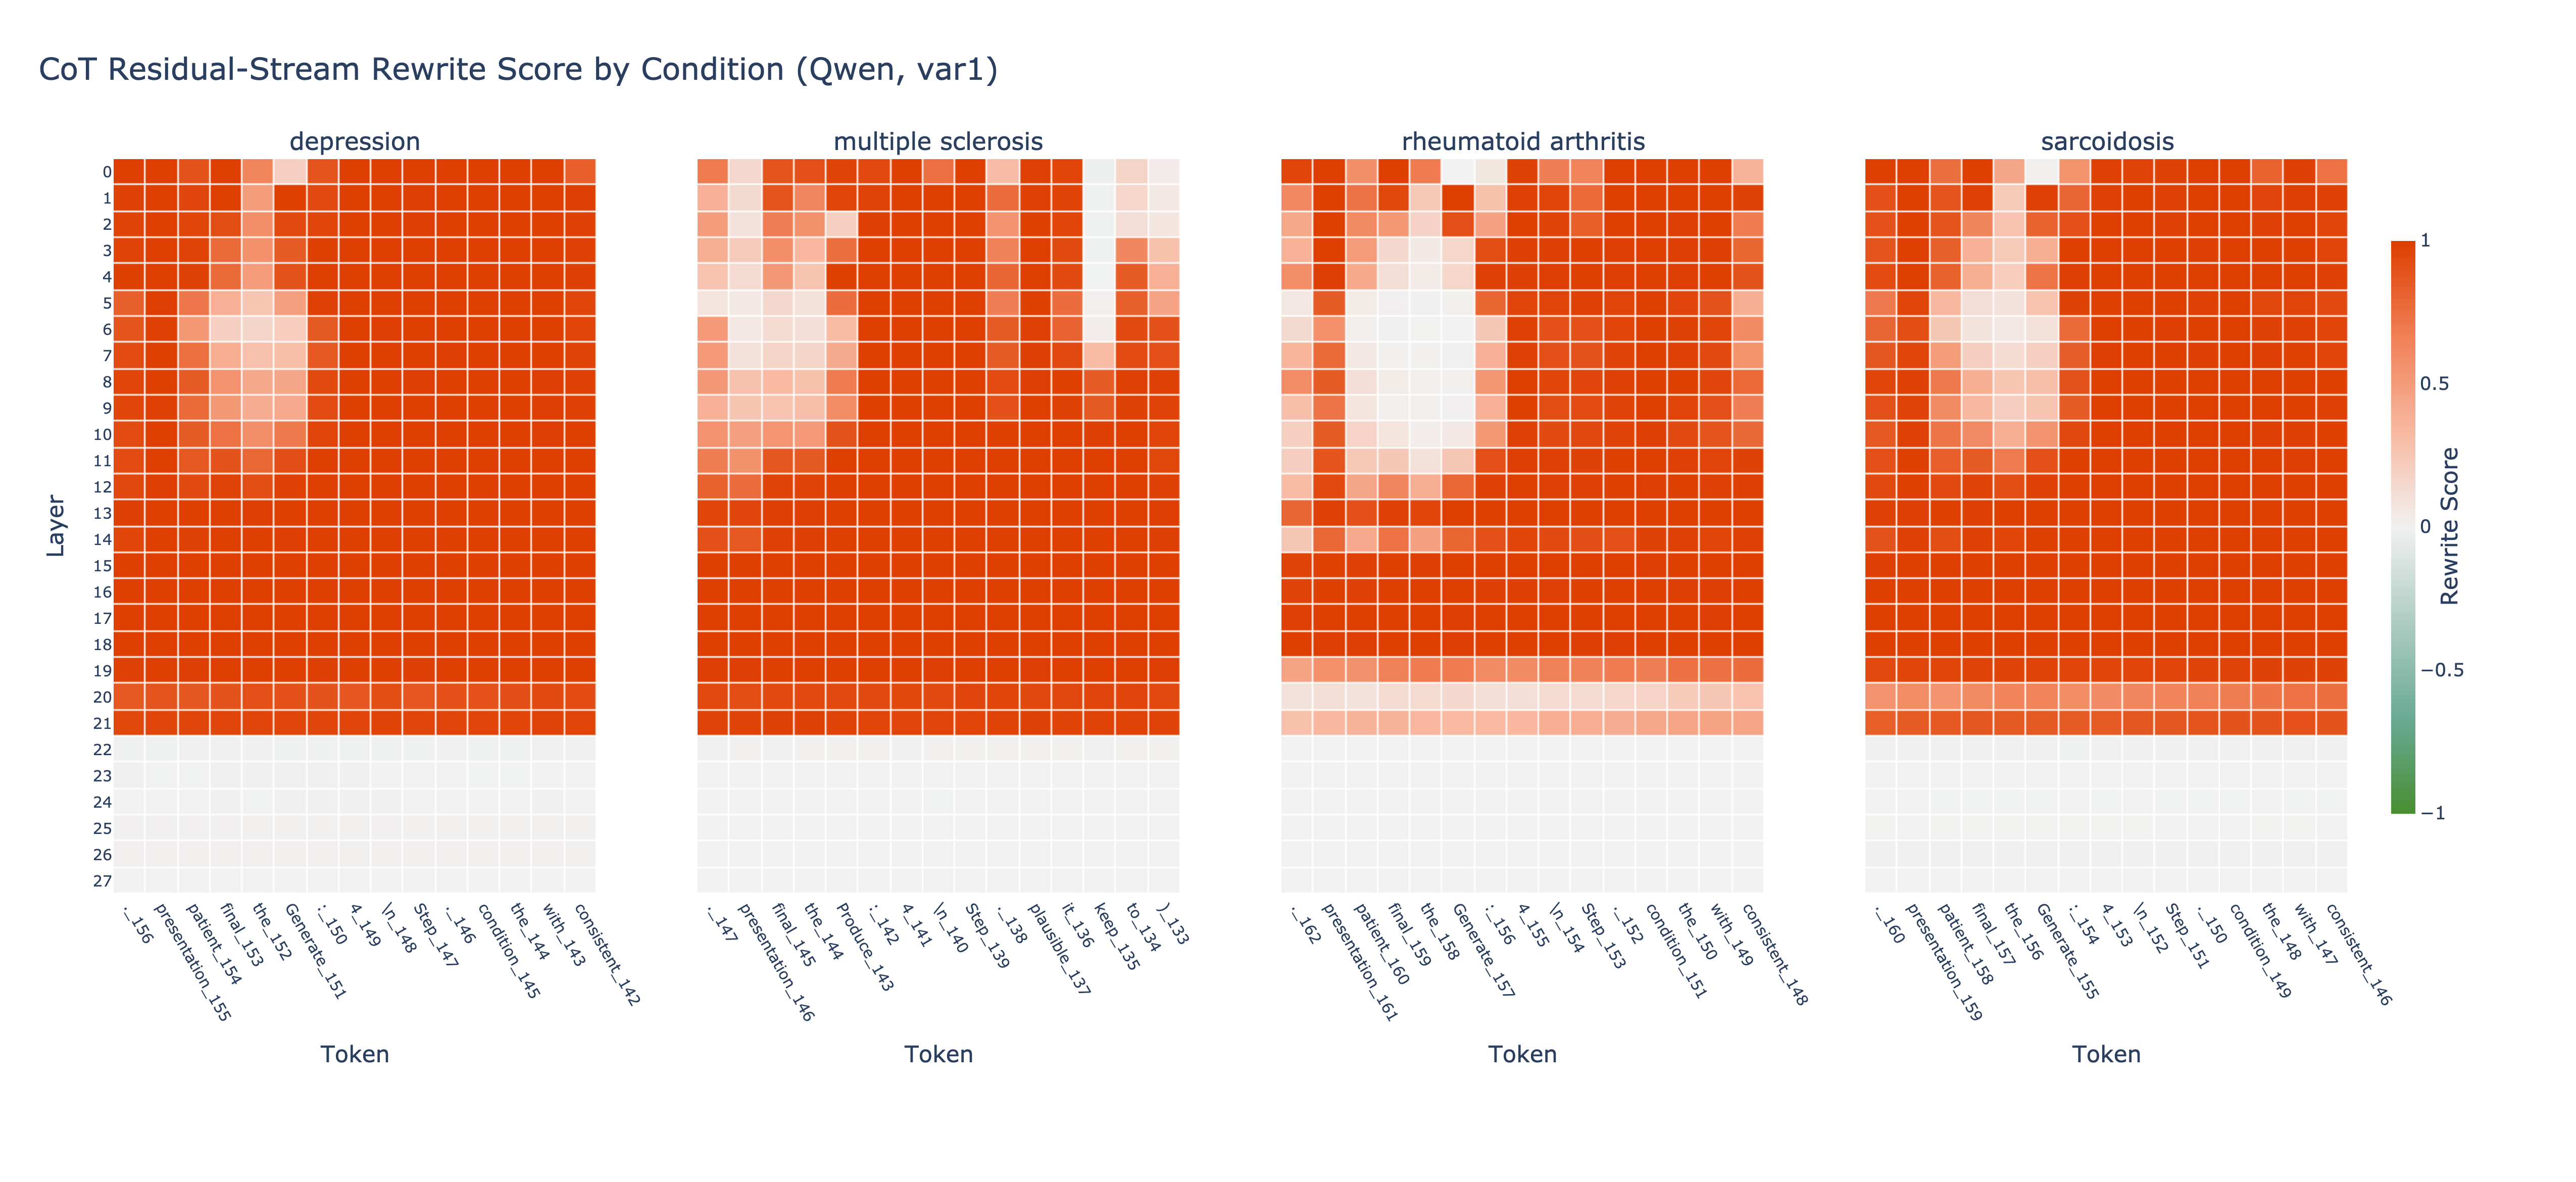
\includegraphics[width=0.7\linewidth]{fig9_cot_residual_by_condition_promptA_var1.png}
    \caption{CoT residual-stream rewrite scores across conditions (Prompt A, var1).}
    \label{fig:cotresid}
\end{figure}
\clearpage

\section{Condition-specific heatmaps for simple prompting}
\label{app:heatmaps}

This disparity in rewrite score across conditions can be further seen by analyzing the specific prompt, condition heatmaps (Figure~\ref{fig:heatmap_app}). Results for asthma across all 31 prompts show similar results, strong localized activation at layer 18 that is associated with the condition token. On the other hand, results from rheumatoid arthritis show little to no rewrite score changes in any of the middle layers. Our findings show the internal encodings of gender bias are not uniform across all female biased diseases. The data displays the disparity in how easily different biases can be patched.

\begin{figure}[h]
    \centering
    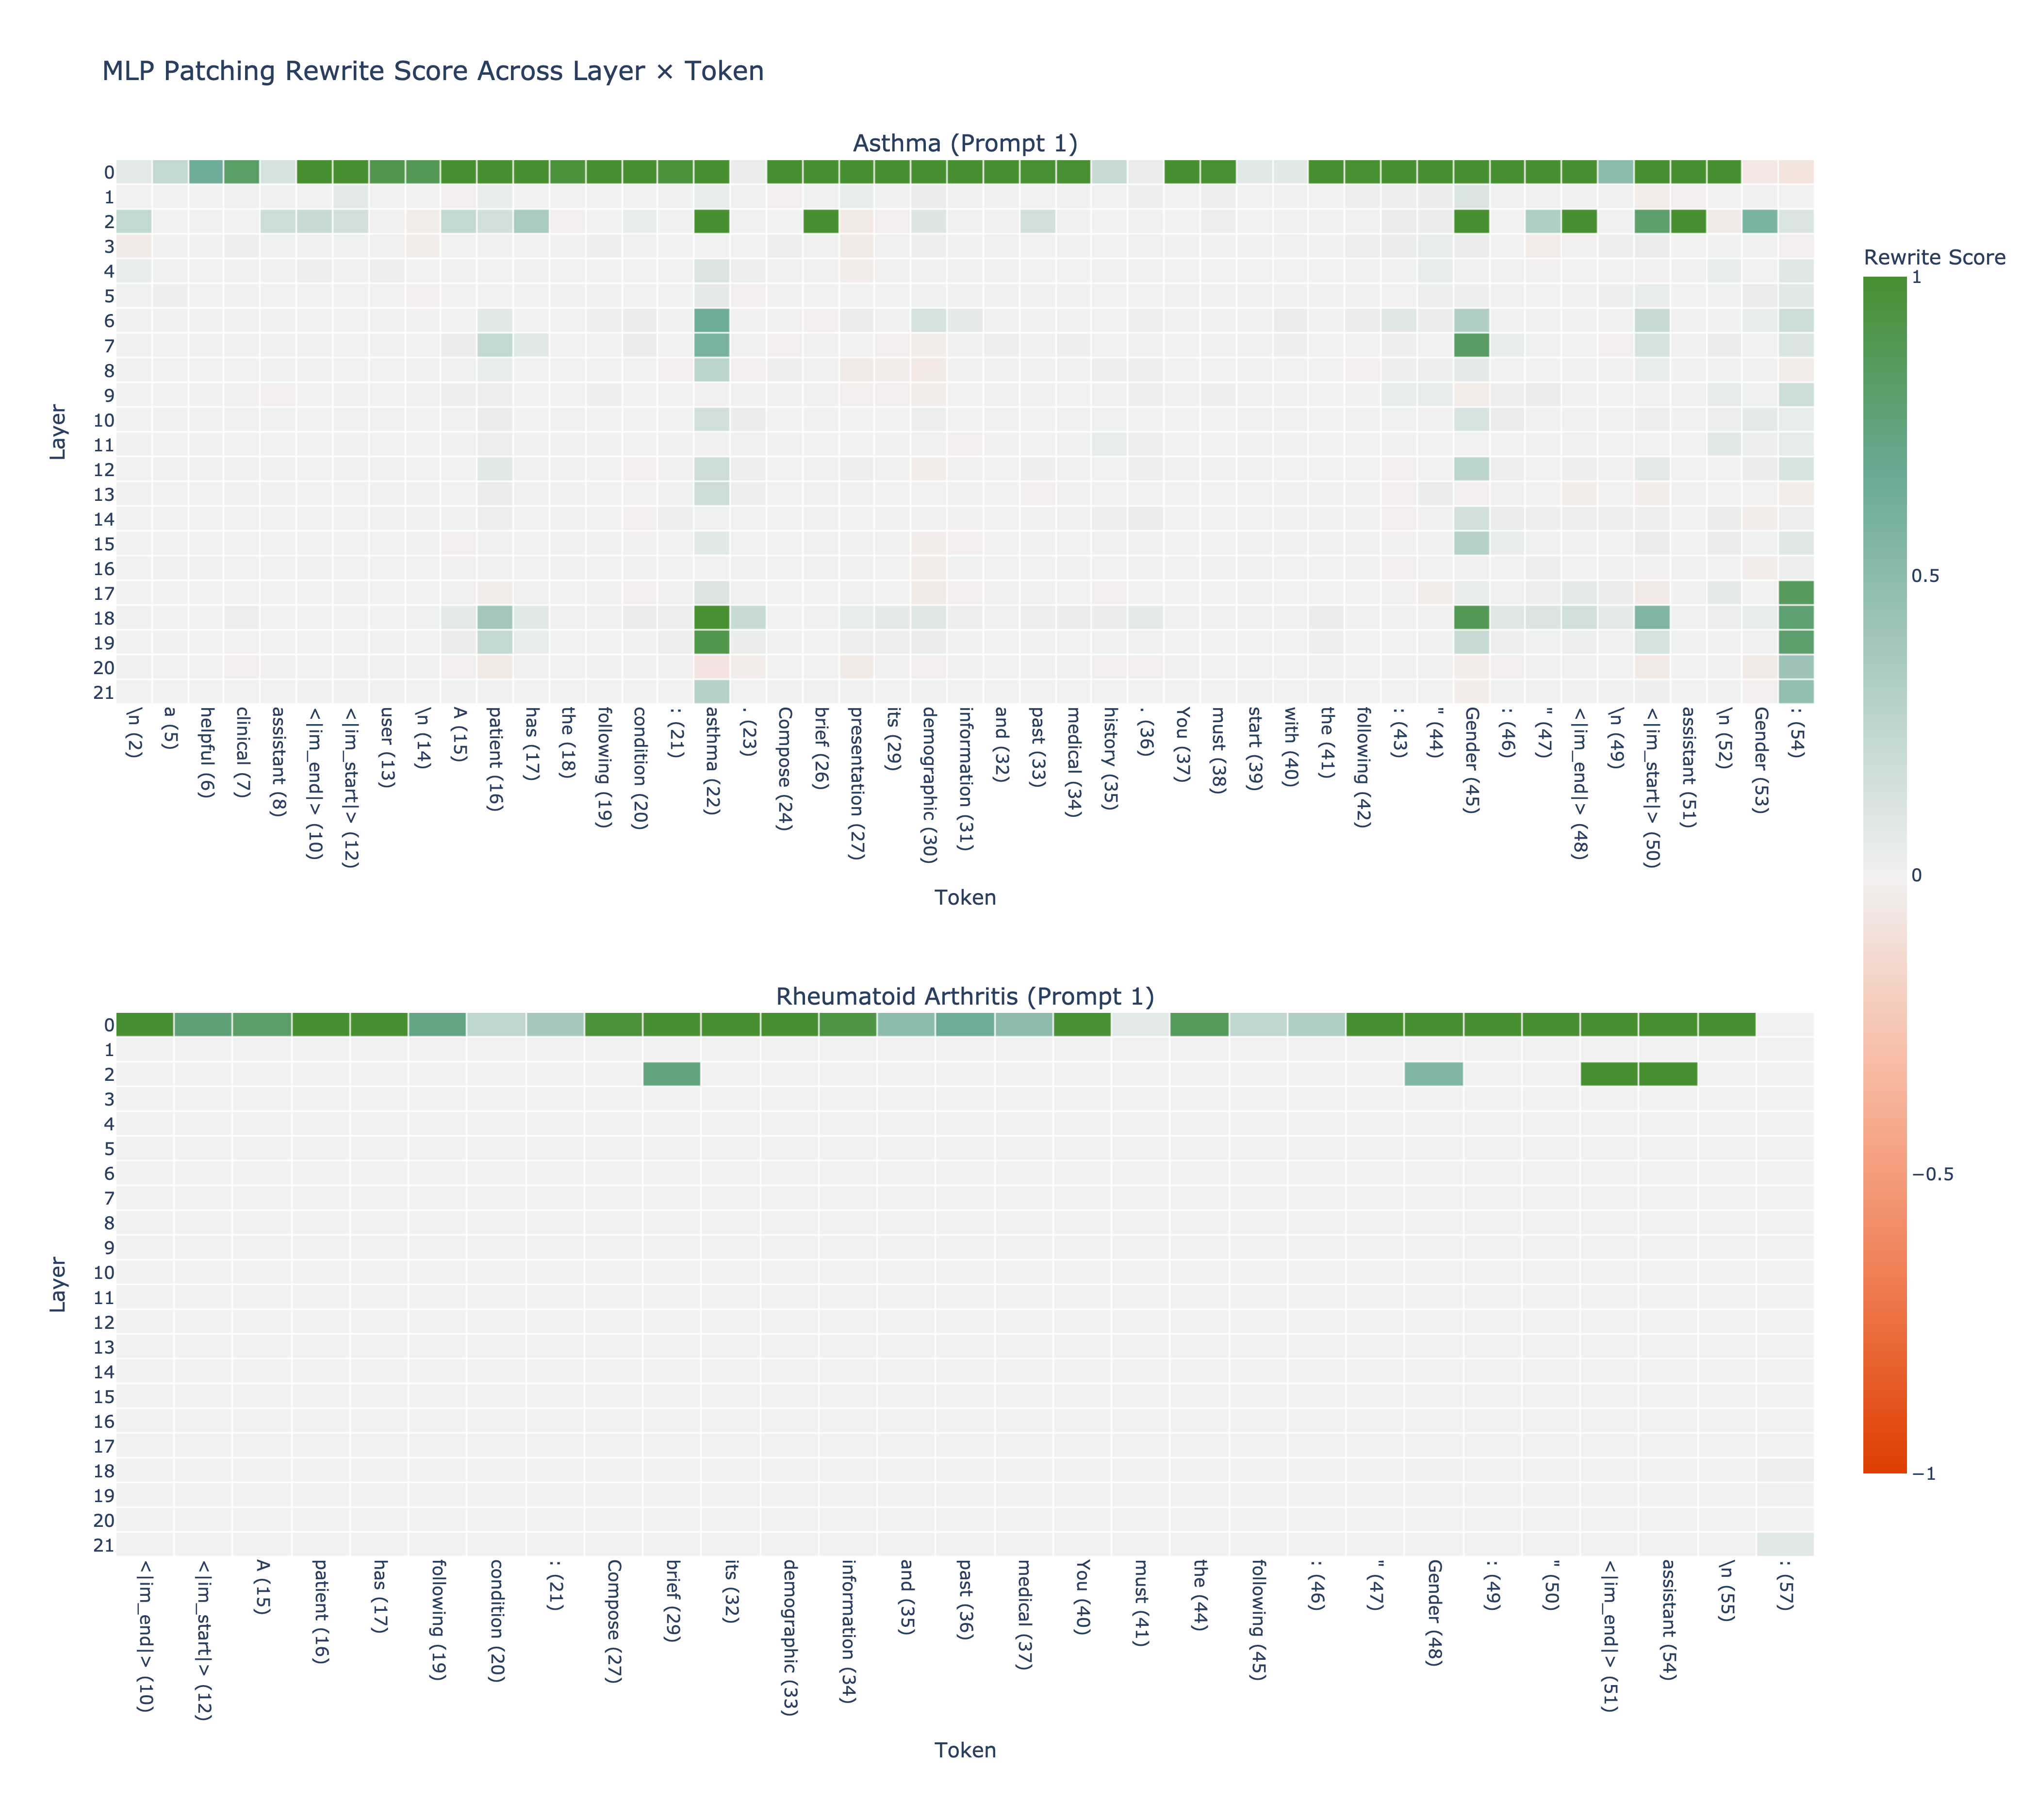
\includegraphics[width=1\linewidth]{fig5_mlp_heatmaps_combined_asthma_ra.png}
    \caption{Qwen simple-prompt MLP patching heatmap (rewrite score) across layer $\times$ token for representative asthma and rheumatoid-arthritis prompts.}
    \label{fig:heatmap_app}
\end{figure}

\clearpage
\section{SAE control comparisons}
\label{app:sae_controls}

To assess whether observed effects reflect causality rather than generic ablation artifacts, we compared real ablations against two control conditions: (1) condition-semantic controls, which ablate latents matched by clinical condition but not identified as gender-biased, and (2) random magnitude-matched controls, which ablate randomly selected latents with similar activation magnitudes.

\begin{figure}[h]
    \centering
    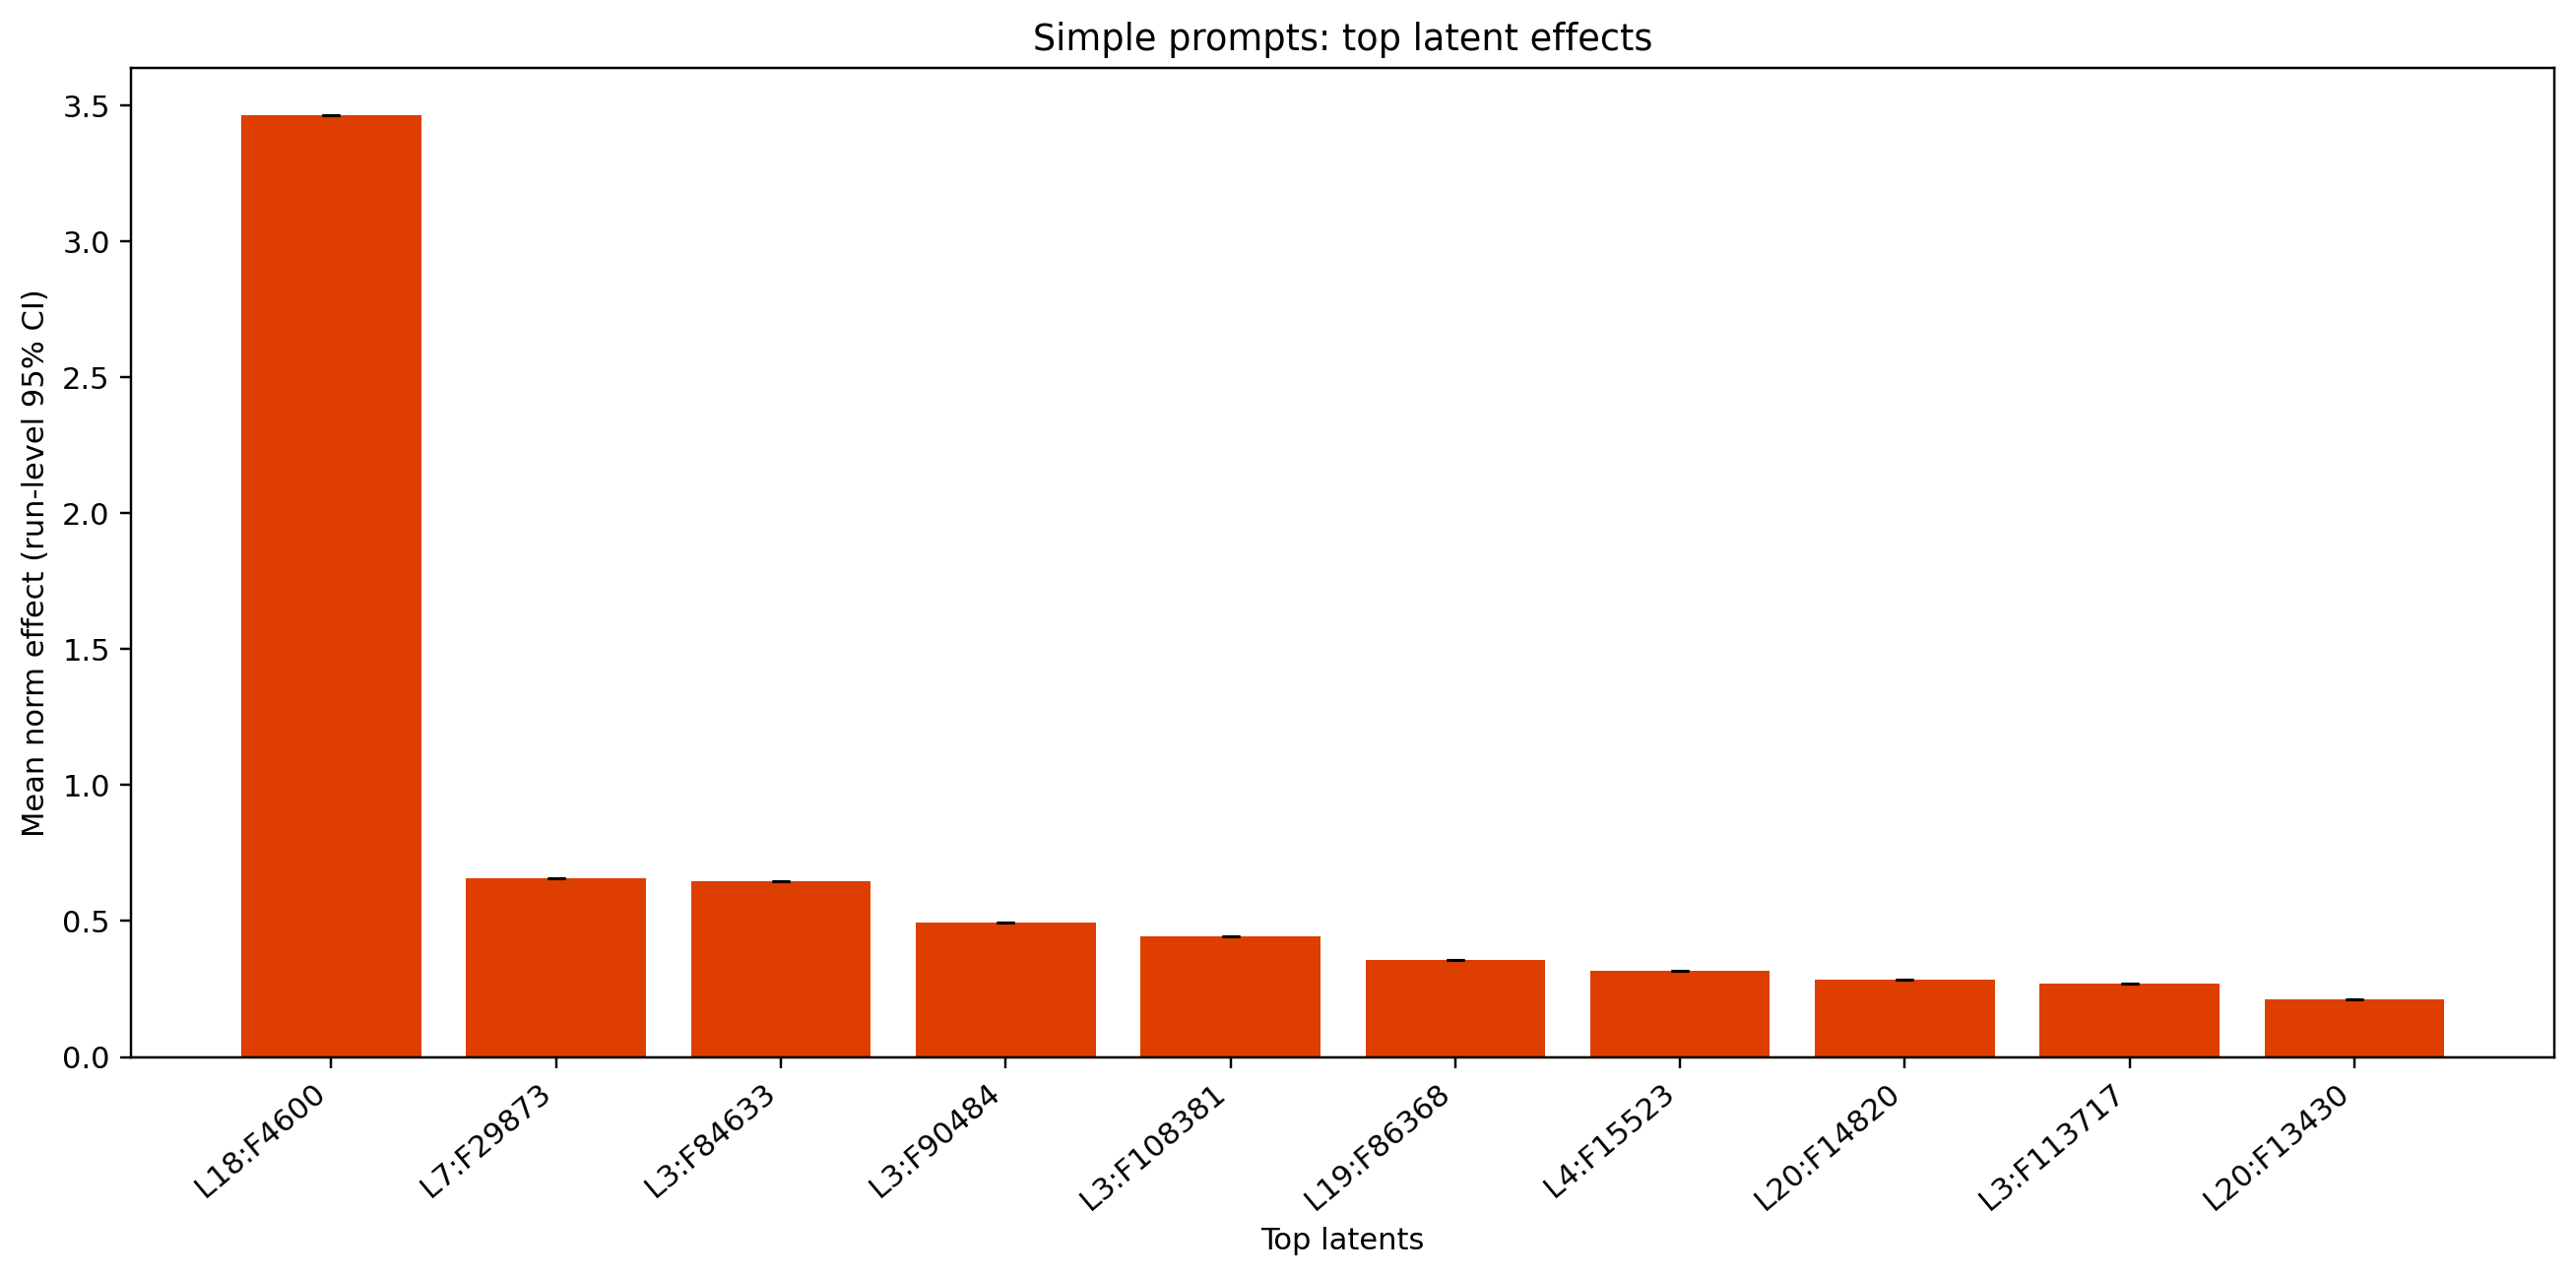
\includegraphics[width=1\linewidth]{fig2_top10_latents_bootstrap_ci_simple.png}
    \caption{SAE top latents mean norm effect scores with 95\% bootstrap confidence intervals for simple prompts.}
    \label{fig:simple_CI}
\end{figure}

\begin{figure}[h]
    \centering
    
\includegraphics[width=1\linewidth]{fig3_real_vs_control_gap.png}
    \caption{SAE real vs control effects on latent ablation (CoT).}
    \label{fig:sae_control}
\end{figure}

\begin{figure}[h]
    \centering
    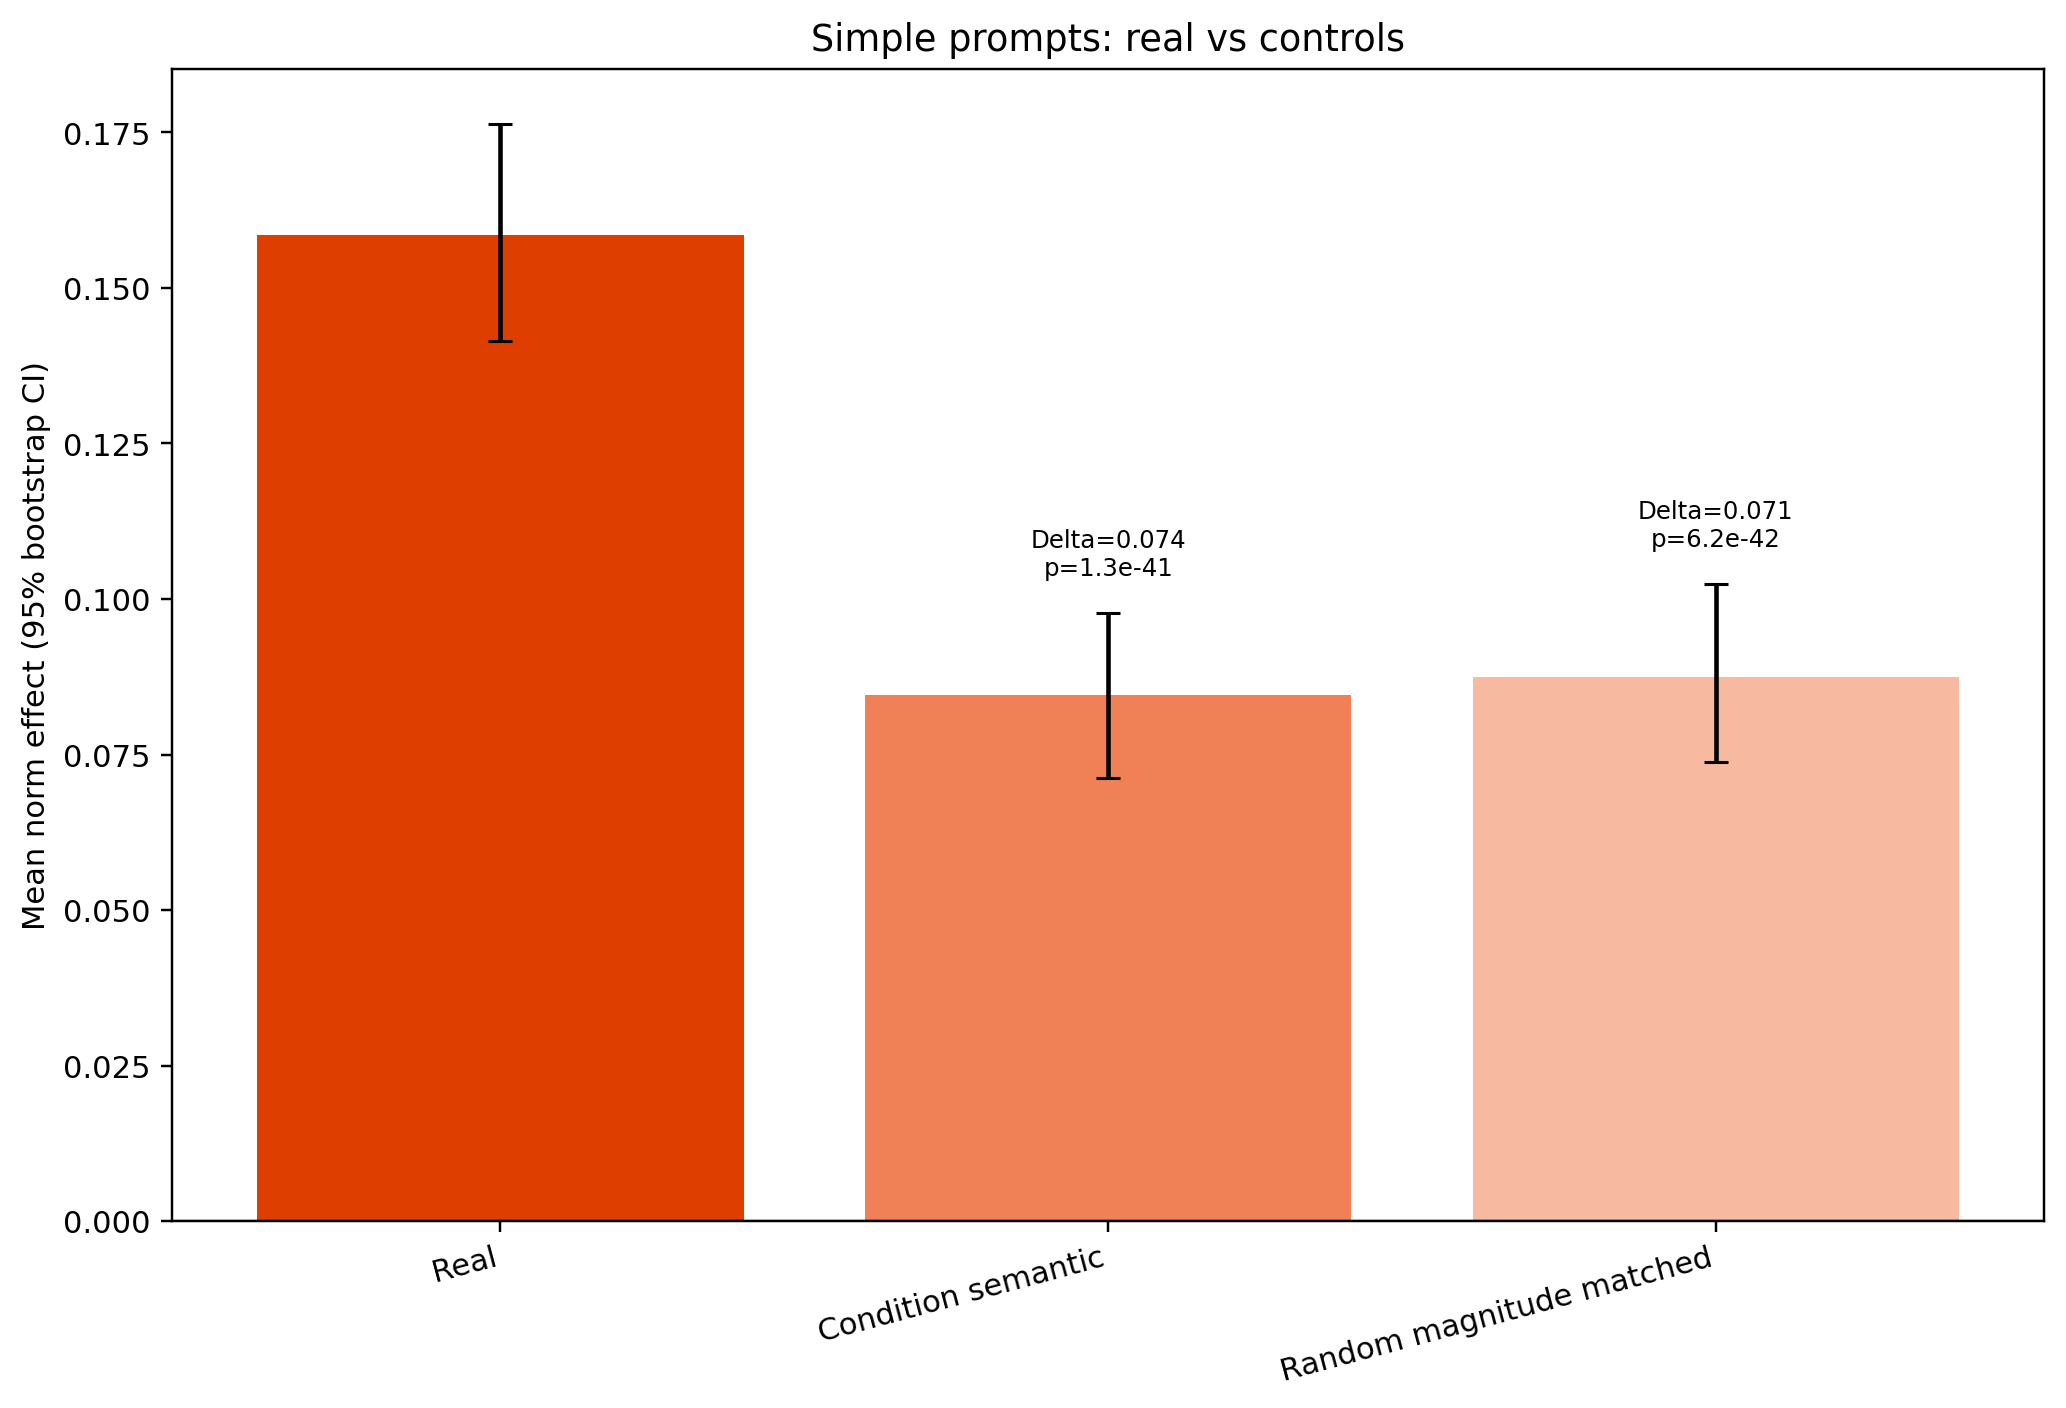
\includegraphics[width=0.9\linewidth]{fig3_ci_real_vs_controls.png}
    \caption{SAE real vs control effects on latent ablation for simple prompts.}
    \label{fig:simple_control}
\end{figure}


\clearpage

\newpage
\input{checklist.tex}

\end{document}
